\documentclass[12pt,a4paper]{amsart}
% ukazi za delo s slovenscino -- izberi kodiranje, ki ti ustreza
\usepackage[slovene]{babel}
%\usepackage[cp1250]{inputenc}
%\usepackage[T1]{fontenc}
\usepackage[utf8]{inputenc}
\usepackage{amsmath,amssymb,amsfonts}
\usepackage{mathrsfs}
\usepackage{url}
%\usepackage[normalem]{ulem}
\usepackage[dvipsnames,usenames]{color}

\usepackage[a-1b]{pdfx}
\hypersetup{pdfstartview=}

\usepackage{graphicx}
\usepackage{algpseudocode}
\usepackage[title]{appendix}

% ne spreminjaj podatkov, ki vplivajo na obliko strani
\textwidth 15cm
\textheight 24cm
\oddsidemargin.5cm
\evensidemargin.5cm
\topmargin-5mm
\addtolength{\footskip}{10pt}
\pagestyle{plain}
\overfullrule=15pt % oznaci predlogo vrstico


% ukazi za matematicna okolja
\theoremstyle{definition} % tekst napisan pokoncno
\newtheorem{definicija}{Definicija}[section]
\newtheorem{primer}[definicija]{Primer}
\newtheorem{opomba}[definicija]{Opomba}

\renewcommand\endprimer{\hfill$\diamondsuit$}


\theoremstyle{plain} % tekst napisan posevno
\newtheorem{lema}[definicija]{Lema}
\newtheorem{izrek}[definicija]{Izrek}
\newtheorem{trditev}[definicija]{Trditev}
\newtheorem{posledica}[definicija]{Posledica}


% za stevilske mnozice uporabi naslednje simbole
\newcommand{\R}{\mathbb R}
\newcommand{\N}{\mathbb N}
\newcommand{\Z}{\mathbb Z}
\newcommand{\CC}{\mathbb C}
\newcommand{\Q}{\mathbb Q}

% ukaz za slovarsko geslo
\newlength{\odstavek}
\setlength{\odstavek}{\parindent}
\newcommand{\geslo}[2]{\noindent\textbf{#1}\hspace*{3mm}\hangindent=\parindent\hangafter=1 #2}

% naslednje ukaze ustrezno popravi
\newcommand{\program}{Finančna Matematika}
\newcommand{\imeavtorja}{Nejc Ševerkar}
\newcommand{\imementorja}{doc. dr. Uroš Kuzman}
\newcommand{\naslovdela}{Mandelbrotova množica in algoritem DEM}
\newcommand{\letnica}{2020}


% vstavi svoje definicije ...
\newcommand{\CCinf} {\hat{\CC}} % razširjena kompleksna ravnina
\newcommand{\D}{\mathbb D} % odprti enotski disk (posplošitev \D_{radij}(sredisce))
\newcommand{\SSS}{\mathbb S} % enotska krožnica (posplošitev \SSS_{radij}(sredisce))
\newcommand{\I}{\mathbb I} % realna enotska krogla (posplošitev \I_{radij}(sredisce))
\newcommand{\M}{\mathscr M} % Mandelbrotova množica
\newcommand{\J}{\mathscr J} % Juliajeve množica (\J^\ast napolnjena Juliajeva množica)
\newcommand{\QQ}{\mathscr Q} % Douady-Hubbard družina kvadratičnih polinomov
\newcommand{\A}{\mathscr A} % baza privlačnosti (v kontekstu)
\newcommand{\E}{\mathscr E} % definicijsko območje Mandelbrot-Bottcher preslikave
\newcommand{\HH}{\mathbb H} % specifično v dokazu
\newcommand{\Real}{\mathrm{Re}}

\newcommand{\Break}{\State \textbf{break} }
\newcommand{\algAnd}{\;\textbf{and}\;}


\begin{document}

% od tod do povzetka ne spreminjaj nicesar
\thispagestyle{empty}
\noindent{\large
UNIVERZA V LJUBLJANI\\[1mm]
FAKULTETA ZA MATEMATIKO IN FIZIKO\\[5mm]
\program\ -- 1.~stopnja}
\vfill

\begin{center}{\large
\imeavtorja\\[2mm]
{\bf \naslovdela}\\[10mm]
Delo diplomskega seminarja\\[1cm]
Mentor: \imementorja}
\end{center}
\vfill

\noindent{\large
Ljubljana, \letnica}
\pagebreak

\thispagestyle{empty}
\tableofcontents
\pagebreak

\thispagestyle{empty}
\begin{center}
{\bf \naslovdela}\\[3mm]
{\sc Povzetek}
\end{center}
% tekst povzetka v slovenscini
V nalogi je predstavljen algoritem {\em DEM (Distance Estimation Method)},
 ki omogoča učinkovito grafično prikazovanje fraktalnih množic. 
Algoritem sodi na področje kompleksne dinamike, ki preučuje obnašanje iteracij kompleksnih preslikav. 
Začetek te veje matematike sega v obdobje med letoma 1917 in 1919,
ko so bile objavljene prve raziskave na temo iteracij kompleksnih racionalnih funkcij ene spremenljivke s strani francoskih matematikov {\em Gastona Juliaja} in {\em Pierre Fatouja}. 
Sledilo je obdobje daljšega mirovanja teorije, ki pa ga je prekinil razvoj numerične matematike in posledično tudi fraktalne geometrije. 
Tako je področje znova postalo zelo popularno tako med matematiki kot med umetniki.
V središču naloge bo eden izmed najbolj znanih objektov te teorije, tako imenovana {\em Mandelbrotova množica}. 
Gre za podmnožico kompleksne ravnine, ki na svojevrsten način ilustrira družino kvadratnih polinomov s povezano {\em Juliajevo množico}. 
V nalogi bomo podali njeno definicijo in dokazali nekaj njenih topoloških lastnosti.
V ospredju bo dokaz njene povezanosti, ki nam bo v zadnjem poglavju omogočil izpeljavo algoritma DEM, 
s katerim bomo to množico tudi učinkovito grafično prikazali.

\vfill
\begin{center}
{\bf The Mandelbrot set and the DEM algorithm}\\[3mm] % prevod slovenskega naslova dela 
{\sc Abstract}
\end{center}
% tekst povzetka v anglescini
The thesis presents the {\em DEM (Distance Estimation Method)} algorithm, 
which enables efficient graphical representation of fractal sets. 
The algorithm belongs to the field of complex dynamics, 
which studies the behavior of iterations of complex mappings. 
The beginnings of this branch of mathematics date back to the period between 1917 and 1919, 
when the first research on the iteration of complex rational functions of one variable was published by the French mathematicians {\em Gaston Julia} and {\em Pierre Fatou}. 
This was followed by a period of prolonged dormancy of the theory, 
which was interrupted by the development of numerical mathematics and consequently also fractal geometry. 
Thus, the field again became very popular among both mathematicians and artists.
At the heart of the thesis will be one of the most famous objects of this theory, the so-called {\em Mandelbrot set}. 
This is a subset of a complex plane that in a unique way illustrates a family of square polynomials with a connected {\em Julia set}. 
In the thesis its definition will be given and some of its topological properties will be proven. 
In the foreground will be the proof of its connectedness, which in the last chapter will make it possible to derive the DEM algorithm, 
using which this set will also be efficiently graphically represented.

\vfill\noindent
{\bf Math. Subj. Class. (2010):} 37F10  \\[1mm]  
{\bf Ključne besede:} kompleksna dinamika, polinomi, Juliajeve množice, Mandelbrotova množica, algoritem \\ [1mm]  
{\bf Keywords:} complex dynamics, polynomials, Julia sets, the Mandelbrot set, algorithm
\pagebreak


% tu se zacne tekst seminarja

\section{Uvod}

Beseda {\em fraktal} opisuje množice, ki obdržijo svojo kompleksno in grobo strukturo na poljubni bližini. 
Ena od njihovih ključnih značilnosti je samopodobnost, torej lastnost množic, pri katerih so njeni manjši kosi podobni celotni množici.
Tipično to pomeni, da njihov rob ni predstavljiv v običajnem grafičnem smislu, temveč se pri njegovi ilustraciji zanašamo na upodabljanje, 
ki je zgolj do želene povečave natančno. Pri slednjem se praviloma zanašamo na numerične algoritme, ki lahko s precejšnjo natančnostjo določajo,
ali je dana točka del fraktalske notranjosti oziroma zunanjosti. 
V delu diplomskega seminarja bomo predstavili tovrstni algoritem {\em DEM (angl. Distance Estimation Method)}, 
s katerim bomo upodobili tako imenovano {\em Mandelbrotovo množico}. Gre za eno izmed najbolj znanih množic te vrste,
ki je poimenovana po snovalcu besede fraktal. Ta množica bo torej v središču naloge, 
izpeljavo algoritma DEM pa nam bo omogočil klasični dokaz njene povezanosti, 
ki sta ga leta 1982 objavila {\em Adrien Douady} in {\em John Hubbard}  (Izrek \ref{izr:DouadyHubbard}).

Teorija, ki je v ozadju definicije Mandelbrotove množice in posledično algoritma DEM, 
ima korenine v veji matematike, poimenovani kompleksna dinamika. 
Ta obravnava obnašanje kompleksnih preslikav pod zaporednimi iteracijami.
Njeni začetki segajo v leto 1915, ko je Francoska akademija znanosti naznanila podelitev nagrade {\em Grand Prix des Sciences Mathematiques} za študijo iteracij kompleksnih funkcij. Vabilu sta se odzvala francoska matematika {\em Gaston Julia} in {\em Pierre Fatou}, ki sta med letoma 1917 in 1919 neodvisno izdala rezultate o iteraciji kompleksnih racionalnih funkcij ene spremenljivke. Njuni rezultati štejejo za temelje kompleksne dinamike, kar je razvidno tudi iz poimenovanja osrednjih objektov v teoriji.

Ker bo naše razumevanje kompleksne dinamike ključno za obravnavo osrednjega objekta te naloge, bomo osnovam te teorije posvetili prvo poglavje. V njem definiramo osnovne iteracijske pojme, kot so {\em orbita}, {\em fiksna točka}, {\em n-cikel} in {\em privlačnost}. Nadalje za razumevanje pojma Mandelbrotova množica potrebujemo razumevanje dinamike kvadratnih polinomov. Skupaj z linearnim primerom jo predstavljamo v drugem poglavju. Eden njegovih ciljev je dokazati, zakaj je teorija lineanih polinomov tako zelo enostavna, da se z njo po navadi ne ukvarjamo. Prava dinamika se namreč začne s polinomi druge stopnje, ki jih do konjugacije natančno pooseblja {\em Douady-Hubbardova družina} polinomov $q_c(z) = z^2 + c$, za $c\in\CC$. Osrednja tema tretjega poglavja bodo {\em B{\"o}ttcherjeve koordinate}, ki omogočajo učinkovito obravnavo dinamike v okolici superprivlačnih točk. Pri tem si bomo ogledali nekaj pomembnih lastnosti te preslikave in pokazali, da je ta teorija izredno pomembna pri študiju polinomske dinamike. V četrtem poglavju bomo spoznali razred množic, ki jih imenujemo {\em Juliajeve množice}. Te imajo v kontekstu polinomov zelo enostavno karakterizacijo, njihova uprizoritev pa bo stranski produkt analize Mandelbrotove množice. Glavni izrek v tem poglavju bo tako imenovana {\em Osnovna dihotomija}, na kateri temelji motivacija definicije Mandelbrotove množice. Končno bomo v istem poglavju prišli še do Mandelbrotove množice, za katero bomo dokazali nekaj osnovnih lastnosti. Naš osrednji cilj pa bo dokaz njene povezanosti s pomočjo tako imenovane {\em Mandelbrot-B{\"o}ttcherjeve preslikave}. Nazadnje bomo v sklepnem poglavju predstavili tudi algoritem DEM, s katerim lahko s pomočjo preslikave prejšnjega poglavja učinkovito upodobimo Mandelbrotovo množico. Z malo truda pa bomo pokazali, da algoritem lahko prilagodimo tudi za upodabljanje Juliajeve množice različnih polinomov.

Tekom naloge bomo predpostavili poznavanje osnovnih rezultatov kompleksne analize in splošne topologije.
Bralec lahko le te poišče v virih \cite{conway} in \cite{kelley}.
Vse slike so avtorske; izdelane so s programskim jezikom {\em Python} in 
pomočjo prostodostopnih paketov {\em Numpy} in {\em Matplotlib}.

\clearpage


\section{Iteracijske osnove}
V prvem poglavju bomo spoznali osnovno teorijo, potrebno za analizo dinamike kompleksnih polinomov.
Le ta vključuje pojme kot so {\em iteracija}, {\em fiksne točke} in {\em n-cikli}.
Čeprav se bomo v nadaljevanju osredotočili le na polinome, bodo definicije v tem razdelku podane za meromorfne funkcije. 
To so funkcije, ki so holomorfne povsod razen v diskretni množici polov. 
Znano je, da lahko take funkcije tretiramo tudi kot holomorfne preslikave, 
ki Riemannovo sfero $\CCinf=\CC\cup\{\infty\}$ preslikajo samo vase. 
Skozi nalogo bomo odprt enotski disk $\{z \in \CC \mid |z| < 1\}$ označevali z $\D$, enotsko krožnico $\{z \in \CC \mid |z| = 1\}$ pa z $\SSS$.
Disk oziroma krožnico s središčem v točki $a\in\CC$ in radijem $r>0$ bomo označevali z $\D_r(a)$ in $\SSS_r(a)$, 
ter z $\D_r$ in $\SSS_r$, ko bo $a=0$.  

\begin{definicija}
Naj bo $U \subset \CCinf$ odprta množica, $f\colon U\to U$ kompleksna funkcija in $a\in U$.
\emph{Iteracijsko zaporedje} funkcije $f$ v točki $a$ je podano s členi
\begin{equation*}
\begin{aligned}
z_0 &= a \\
z_n &= f(z_{n-1}) = f^n(z_0).
\end{aligned}
\end{equation*}
\end{definicija}

\noindent Zaporedju $(f^n(a))_n$ rečemo tudi {\em orbita} točke $a$.

\begin{figure}[h]
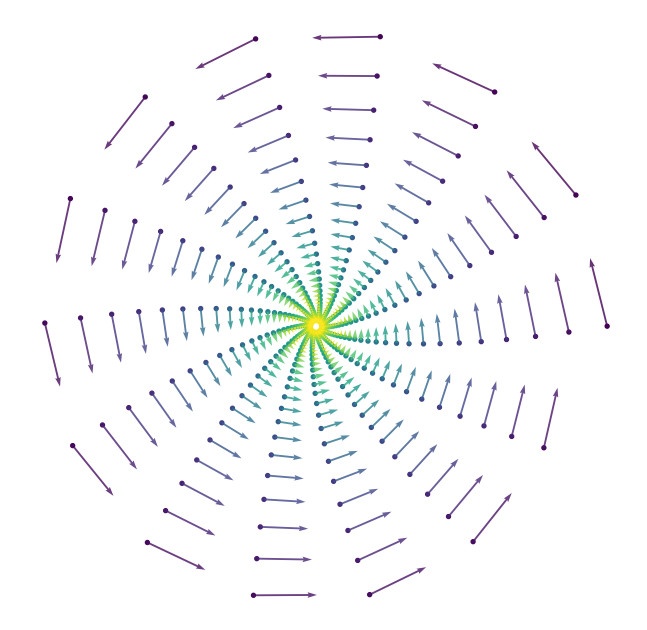
\includegraphics[width=6cm]{graphics/orbitaQuiver3.jpg}
\caption{
Orbita iteracije $(z \to 0.99 \exp(\sqrt{0.2}i)z)$ z začetkom v $a=1$.
Puščice označujejo smer premika orbite, medtem ko
modra barva opisuje zgodnje, rumena pa pozne člene.
}
\end{figure}

\begin{definicija}\label{def:fixedPoint}
Točki $\alpha\in U$, za katero velja $f(\alpha)=\alpha$, pravimo {\em fiksna}.
\end{definicija}

\begin{definicija}\label{def:nCycle}
Naj bo $f \colon U \to U$ in $n \in \N$. Pravimo, da nabor $(u_1, u_2, \dots, u_n)$ tvori {\em$n$-cikel}, 
če je $n$ najmanjše takšno število, da veljata lastnosti
\begin{equation*}
\begin{aligned}
f(u_i) &= u_{i+1} \quad \text{za} \quad  i < n, \\
f(u_n) &= u_1.
\end{aligned}
\end{equation*}
\end{definicija}

\noindent Fiksne točke imajo v iteracijah posebno vlogo, 
saj se iteracija na njih ustavi oziroma ima konstantno orbito. 
Naslednja trditev nam bo opisala tudi pomembno lastnost fiksnih točk,
ki pravi, da so te točke edine možne limite elementov posameznih orbit.

\begin{trditev}\label{trd:fixedPointConvergance}
Naj bo dana zvezna funkcija $f \colon U \to U$. 
Če obstaja takšen $a \in U$, da je zaporedje $(f^n(a))_n$ konvergentno z limito $\alpha$,
potem je $\alpha$ {\em fiksna točka} funkcije $f$.
\end{trditev}

\proof
Privzemimo torej, da je $\alpha = \lim_{n \to \infty}f^n(a)$. 
Uporabimo lahko izrek o zamenjavi zvezne funkcije $f$ in limite konvergentnega zaporedja $(f^n(a))_n$ in tako dobimo
$$f(\alpha) = f(\lim_{n \to \infty} f^n(a)) = \lim_{n \to \infty} f^{n+1}(a) = \alpha.$$
Sklep velja, ker je funkcija $f$ zvezna na $U$ in to množico vedno preslika vase.
\endproof

Vidimo torej, da so fiksne točke naravni kandidati za limite iteracijskih zaporedij.
Seveda pa orbite ne konvergirajo vedno.
Naslednja definicija nam v tem kontekstu karakterizira tip fiksne točke za holomorfno preslikavo.

\begin{definicija}\label{def:fixedPointTypes}
Naj bo dana holomorfna funkcija $f \colon U \to U$ s fiksno točko $\alpha \in U$ in naj bo $\lambda = |f'(\alpha)|$.
Če velja $\lambda < 1$, pravimo, da je $\alpha$ {\em privlačna} fiksna točka, če je $\lambda > 1$, pravimo, da je točka {\em odbojna}, 
če pa je $\lambda = 1$, pa jo imenujemo {\em nevtralna}. 
\end{definicija}

Oglejmo si trditvi, ki bosta pojasnili razlog poimenovanja prvih dveh tipov fiksnih točk.

\begin{trditev}\label{trd:attractionBasin}
Naj bo  $\alpha$ privlačna fiksna točka holomorfne funkcije $f \colon U \to U$. 
Potem obstaja okolica točke $\alpha$, na kateri zaporedje funkcij $(f^n)_n$
po točkah konvergira h konstantni funkciji $\alpha$.
\end{trditev}

\proof
Iz definicije odvoda in privlačne fiksne točke dobimo $|\lim_{z \to \alpha} \frac{f(z) - \alpha}{z - \alpha}| < 1$.
Za nek $\varepsilon > 0$, $|z - \alpha| < \varepsilon$ in $0 \leq \lambda < 1$ potem velja
\begin{equation*}
\begin{aligned}
|f(z) - \alpha| & \leq \lambda |z  - \alpha| \\
|f^n(z) - \alpha| &\leq \lambda^n |z - \alpha| \\
|f^n(z) - \alpha| &< \lambda^n \varepsilon.
\end{aligned}
\end{equation*}
Ker aproksimacija velja za vse elemente $z \in \D_\varepsilon(\alpha) = \{z + \alpha \mid z \in \D_\epsilon\}$, 
na tem območju sledi konvergenca funkcijskega zaporedja $(f^n)_n$.
\endproof

\begin{opomba}\label{op:attBasinOpen}
Trditev nam zagotovi obstoj posebne okolice $V$ privlačne fiksne točke $\alpha$, 
za katero velja, da orbite vseh elementov iz $V$ konvergirajo k $\alpha$.
Unijo vseh takšnih okolic imenujemo {\em baza privlačnosti} ter jo označimo z $\A_\alpha$.
Velja zveza
$$\A_\alpha = \bigcup_{n\in\N} f^{-n}(V).$$
Ker je $f$ zvezna, sledi, da je baza privlačnosti $\A_\alpha$ odprta.
\end{opomba}

\begin{figure}[h]

\includegraphics[width=5cm]{graphics/attractionBasin.png}
\caption{Baza privlačnosti za točko $3/8$ iteracije $z \to z^2 + 15/64$.}
\end{figure}

Opazimo torej, da je obnašanje orbite dovolj blizu privlačne fiksne točke natanko določeno in predvidljivo.
Poglejmo obnašanje še v primeru odbojnih fiksnih točk.

\begin{trditev}
Naj bo $\alpha$ odbojna fiksna točka holomorfne funkcije $f \colon U \to U$.
Potem obstaja okolica $\alpha$, za katero velja, da vsaka orbita, ki se začne v njej,
po končno korakih izstopi iz nje, če le začetni člen ni enak $\alpha$.
\end{trditev}

\proof
Ker $|\lim_{z\to\alpha}\frac{f(z) - \alpha}{z - \alpha}| > 1$, lahko za nek $\varepsilon > 0$
poiščemo takšen $\lambda > 1$, da velja 
$$|f(z) - \alpha| \geq \lambda |z - \alpha|$$
za vse $z \in \D_\varepsilon(\alpha)$.
Recimo torej, da začnemo z orbito v $w \in \D_\varepsilon(\alpha) \smallsetminus \{\alpha\}$.
Poiščimo takšen $n\in\N$, da je $\lambda^n |w - \alpha| > \varepsilon$. 
Če obstaja takšno naravno število $k < n$, da zanj velja $f^k(w) \notin \D_\varepsilon(\alpha)$, smo dokaz zaključili, sicer pa dobimo
$$|f^n(w) - \alpha| \geq \lambda^n|w - \alpha|  > \varepsilon,$$ 
torej $f^n(w) \notin \D_\varepsilon(\alpha)$.
\endproof

\begin{posledica}\label{pos:odbojnaKonv}
Naj bo $\alpha$ odbojna fiksna točka holomorfne funkcije $f \colon U \to U$.
Če za nek $w \in \CC$ velja $\lim_{k\to\infty} f^k(w) = \alpha$, potem obstaja takšen $n\in\N$,
da $f^n(w) = \alpha$.
\end{posledica}

\begin{primer}\label{pr:LinearDynamicsIntro}
Poglejmo si preslikavo $z \to \lambda z$, kjer $\lambda\in\mathbb{C}\smallsetminus\{0\}$.
Takoj opazimo, da je izhodišče njena edina fiksna točka. 
Nadalje velja, da je ta točka privlačna, če je $|\lambda| < 1$,
odbojna, če je $|\lambda| > 1$ in nevtralna, če je $|\lambda| = 1$.
Geometrijska zasnova te preslikave je zelo enostavna, 
saj gre zgolj za rotacijo za kot $\textrm{arg}(\lambda)$ in razteg oz. skrčitev za faktor $|\lambda|$. 
Zato velja, da bodo v prvem primeru iteracije v poljubni točki $z$ konvergirale proti izhodišču,
saj se bo njihova absolutna vrednost zmanjševala.
V drugem primeru bo konvergenca podobna, a proti točki $\infty$ z omejitvijo $z\neq0$.
V tretjem pa bo ali vsaka točka ciklična ali pa bo edina ciklična točka fiksna točka v izhodišču.
Vse tri primere bomo še nekoliko podrobneje obravnavali v naslednjem poglavju.

\begin{figure}[h]
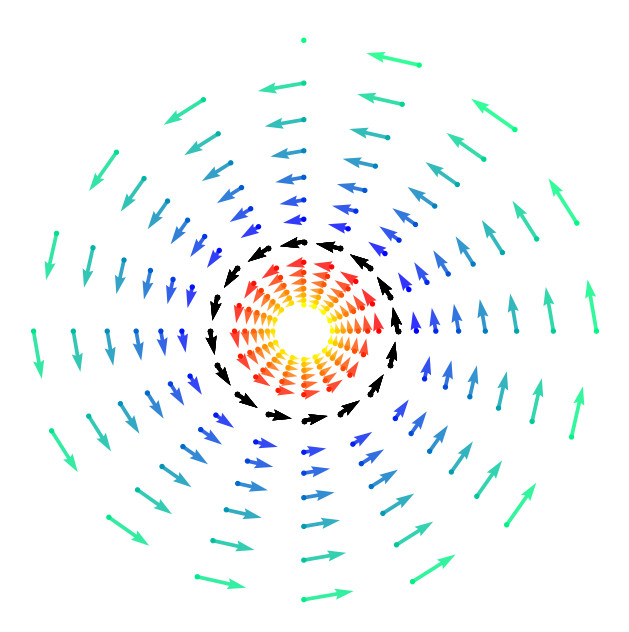
\includegraphics[width=6cm]{graphics/LinearOrbitTrichotomy2.jpg}
\caption{
Slika orbit $z \to \lambda z$ pri treh vrednostih $\lambda$.
Za $a = \exp(\pi i / 8)$ rdeča barva prikazuje primer $\lambda = 0.99 a$ v začetni točki $0.8$,
modra primer $\lambda = 1.01 a$ v začetni točki $1.2$, 
črna pa primer $\lambda = a$ v začetni točki $1$.
}
\end{figure}
\noindent Pripomnimo še, da so obnašanja na zgornji sliki neodvisna od začetnih točk.
\end{primer}
\vskip 2mm

Oglejmo si še nekaj primerov in trditev za funkcije z $n$-cikli.
Slednje bomo iskali preko dejstva, da je vsaka točka na $n$-ciklu fiksna točka za funkcijo $f^n$.
Seveda pa moramo pri tem preveriti, da ne gre že za cikel manjše dolžine oziroma celo za fiksno točko.
Za začetek si oglejmo primer, ki nakaže, da število ciklov ni nujno končno.

\begin{primer}
Vzemimo preslikavo $f \colon z \to 1/z$.
Fiksni točki sta dve in sicer točki $z=\pm1$. Nadalje poiščimo $2$-cikle.
To storimo s pomočjo fiksnih točk funkcije $f^2 \colon z \to z$.
Ker je vsaka točka fiksna za identično preslikavo, sledi, da so $2$-cikli natanko oblike $(u, 1/u)$ za $u \in \CC \smallsetminus \{1, -1\}$.
\end{primer}

\begin{trditev}\label{trd:cycleConvergance}
Naj bo $f \colon U \to U$ zvezna in $\{u_1, u_2, \dots, u_n\} \subset U$. Če velja 
$$\lim_{k\to\infty}f^{kn + j} (z) = u_j$$
za $1 \leq j \leq n$ in nek $z\in U$, potem je $(u_1, u_2, \dots, u_m)$ $m$-cikel za $f$ in nek $m | n$.
\end{trditev}

\proof
Podobno kot v dokazu Trditve \ref{trd:fixedPointConvergance} upoštevamo zveznost $f$ na $U$
$$f(u_j) = f(\lim_{k\to\infty} f^{kn + j} (z)) = \lim_{k\to\infty} f^{kn + (j+1)} (z) = u_{\sigma(j)},$$
kjer je $u_{\sigma(j)}$ enak cikličnemu nasledniku $u_j$ v danem naboru. 
\endproof

Sledi torej, da v primeru, ko lahko stekališča opišemo kot limite ustreznih aritmetičnih podzaporedij orbite, ta tvorijo cikel.

\begin{primer}
Oglejmo si preslikavo $f \colon z \to z^{-2}$. 
Orbito lahko razdelimo na dve podzaporedji s členi
$$f^{2n}(z) = z^{2^{2n}} \quad \text{in} \quad f^{2n+1}(z) = z^{-2^{2n+1}}.$$
Za $|z| > 1$ potem prvo konvergira k $\infty$, drugo pa k $0$. Po Trditvi \ref{trd:cycleConvergance}
dobimo, da par $(0, \infty)$ tvori $2$-cikel za $f$, kar je res, če $f$ zvezno razširimo na $\CCinf$.
\end{primer}

\begin{definicija}
Naj bo $f \colon U \to U$ holomorfna. Za $n$-cikel $(u_1, u_2, \dots, u_n)$ v $U$ pravimo, da je privlačen, če velja
$|f'(u_1) \cdot f'(u_2) \cdot \; \cdots \; \cdot f'(u_n)| < 1$.
\end{definicija}

\begin{opomba}
Če izračunamo odvod holomorfne preslikave $f^n \colon U \to U$ v točki $u_1$ z uporabo verižnega pravila, dobimo
\begin{align*}
(f^n)'(u_1) &= (f^{n-1})'(f(u_1)) \cdot f'(u_1) = (f^{n-1})'(u_2) \cdot f'(u_1) \\
&= f'(u_1)\cdot f'(u_2) \cdot \; \cdots \; \cdot f'(u_n).
\end{align*}
Enak izraz dobimo pri poljubni začetni točki $u_k$ za $1 \leq k \leq n$, 
torej je vrednost odvoda $f^n$ v poljubni točki $n$-cikla enaka tej, ki smo jo uporabili v definiciji.

\noindent Na očiten način s to vrednostjo karakteriziramo tudi odbojne in nevtralne cikle.
\end{opomba}

Za privlačne $n$-cikle lahko podobno kot za fiksne točke karakteriziramo bazo privlačnosti.
To naredimo s pomočjo $n$-te iteracije opazovane preslikave $f$, za katero so točke na privlačnem $n$-ciklu privlačne fiksne.
Torej ima vsaka točka na tem ciklu bazo privlačnosti glede na preslikavo $f^n$.
Posledično na teh območjih ne dobimo nujno zagotovljene konvergence iteracij $f$, 
ampak le konvergenco njihovih aritmetičnih podzaporedij, ki so enake oblike tem iz Trditve \ref{trd:cycleConvergance}.
Ker pa ta podzaporedja opišejo celotno orbito $f$, spet velja, da je njena dinamika na teh okolicah enostavna in natanko določena.



\section{Polinomi prve in druge stopnje}
V tem poglavju se bomo osredotočili na polinome dveh najnižjih stopenj, 
pri katerih je možno analizo dinamike učinkovito prevesti na analizo bolj enostavnih razredov funkcij.
To nam bo med drugim omogočalo podati popolno klasifikacijo dinamike linearnih polinomov,
kar pa bo tudi razlog, da bomo le te v nadaljevanju diplomske naloge zanemarili.
Nasprotno se bo izkazalo, da je prehod iz linearnega v kvadratičen primer zelo netrivialen in da je pri slednjih analiza mnogo bolj zahtevna.

\subsection{Polinomi prve stopnje}
Naj bo $p(z) = az + b$, kjer $a, b \in \CC$.
V primeru, ko je $a = 1$, je dinamika $p$ zelo preprosta, saj je opisana s premiki v smeri $b$ neodvisno od izbire $z$.
Če je $b=0$ je vsaka točka nevtralna fiksna, sicer pa izrazimo
$$p^n(z)=z+nb$$
in dobimo, da za poljubno $z\in\CCinf$ velja $p^n(z)\to\infty$. 
Točka $z=\infty$ je torej edina (privlačna) fiksna točka,  njeno območje privlačnosti pa je celotna sfera $\CCinf$.

Osredotočimo se torej na primere, ko $a \neq 1$. 
Tudi v tem primeru znamo iteracije polinoma izraziti eksplicitno, in sicer kot
$$p^n(z) = a^nz + b\sum_{i = 0}^{n-1}a^i,$$  
a je ta izraz manj primeren za analizo. 
Zato bomo $p$ skušali prevesti na enostavnejšo funkcijo.

\begin{definicija}
Kompleksni funkciji $f \colon U \to U$ in $q \colon V \to V$ sta  {\em konjugirani}, 
če obstaja biholomorfna preslikava $h \colon U \to V$, 
da na $V$ velja $q = h \circ f \circ h^{-1}$. 
Funkcijo $h$ v tem primeru imenujemo {\em konjugacija} med $f$ in $q$ na območjih $U$ in $V$.
\end{definicija}

Konjugacijo uporabljamo za transformacijo med funkcijami,
ki imajo ekvivalentno dinamiko. Natančneje, ob konjugiranju funkcije se nam ohranijo osnovne iteracijske lastnosti.
Če nas na primer zanima obnašanje funkcije $q$ in smo našli biholomorfno preslikavo $h$, 
za katero velja $q = h \circ f \circ h^{-1}$, lahko izrazimo tudi
\begin{equation*}
\begin{aligned}
q^n &= h \circ f \circ h^{-1} \circ h \circ f \circ h^{-1} \circ \dots \circ h \circ f \circ h^{-1} \\
&= h \circ f^n \circ h^{-1},
\end{aligned}
\end{equation*}
s čimer smo iterate funkcije $q$ izrazili z iterati funkcije $f$. 
To nam koristi v primerih, ko je dinamična obravnava iteracij $(q^n)_n$ 
zahtevnejša od iteracij funkcije $f$.
Izkaže se, da konjugacija ohranja tudi tip fiksnih točk, 
saj v primeru, ko je $\alpha$ fiksna točka za holomorfno funkcijo $f$, z verižnim pravilom dobimo
\begin{align*}
&q'(z) = h'(f(h^{-1}(z))) \cdot f'(h^{-1}(z)) \cdot  1 / h'(h^{-1}(z)) \implies q'(h(\alpha)) = f'(\alpha).
\end{align*}
Torej sta fiksni točki $\alpha$ in $h(\alpha)$ za svoji pripadajoči preslikavi enakega tipa.

\begin{trditev}
Naj bo $a \neq 1$. Potem sta polinoma $p(z) = az + b$ in $f_a(z) = az$ konjugirana preko 
biholomorfne preslikave $h\colon\hat{\mathbb{C}}\to \hat{\mathbb{C}},$ podane z $h(z) = z + b / (1 - a)$.
\end{trditev}

\proof
Če opazimo, da velja $h^{-1}(z) = z - b / (1 - a)$, lahko brez težav izpeljemo enakost
$h \circ f_a \circ h^{-1} (z) = p(z)$, s čimer pa je trditev dokazana.
\endproof

Zgornja trditev pove, da lahko namesto dinamike preslikave $z \to az + b$ preučujemo dinamiko preslikave
$$f_a \colon z \to az,$$
ki smo jo obravnavali že v Primeru \ref{pr:LinearDynamicsIntro}.
Iteracije slednje so mnogo preprostejše, saj imajo obliko $f_a^n(z) = a^nz$,
dinamika poljubne točke $z\neq0$ pa je odvisna le od kompleksnega števila $a$. 
Pogledali si bomo obnašanje teh iteracij za vse $a\in\CC\smallsetminus\{0\}$. 
Kot že ugotovljeno, v dveh osnovnih primerih dobimo dinamiko, v kateri vse razen ena točka na sferi konvergirajo k privlačni fiksni točki.
In sicer
\begin{enumerate}
\item ko $|a|> 1$, velja $\lim_{n\to\infty}f_a^n(z) = \infty$ neodvisno od $z \neq 0$,
\item ko $|a| < 1$, velja $\lim_{n\to\infty}f_a^n(z) = 0$ neodvisno od $z \neq \infty$.
\end{enumerate}
Preostane nam še tretji, nekoliko težji primer, ko je $|a| = 1$ in $a\neq 1$. 
Tu je dinamika zanimivejša, čeprav velja, da za poljubno začetno točko iteracije $z_0$ orbite ležijo na
krožnici $\SSS_{|z_0|}$ s središčem v izhodišču in polmerom enakim $|z_0|.$ 
In sicer se izkaže, da moramo obravnavati dva tipa dinamičnega obnašanja glede na njihov polarni zapis $a=e^{i \theta_a}$.
Če je $\theta_a$ racionalni večkratnik $2\pi$, potem obstaja par števil $(q, n) \in \Z \times \N$, 
za kateri je $\theta_a = 2 \pi q / n$. Enostavno je preveriti, da tedaj velja enakost $a^nz = z$.
Če privzamemo, da sta $q$ in $n$ še tuji, je dinamika $q_a$ opisana z nevtralnim $n$-ciklom $(z, az, a^2z, \dots, a^{n-1}z)$.
Preostanejo nam še $a \in \SSS$, za katere je $\theta_a$ iracionalni večkratnik $2\pi$.
Dinamiko tega primera karakterizira {\em Jacobijeva lema}.

\begin{lema}[Jacobijeva lema]\label{lema:Jacobi}
Naj bo $a = e^{i\theta_a}$, kjer je $\theta_a$ iracionalni večkratnik števila $2\pi$. 
Potem je orbita iteracije $z \to az$ v poljubni točki $z_0$ gosta na $\SSS_{|z_0|}$.
\end{lema}

\proof
Predpostavimo torej, da je $\theta_a = 2r\pi$ za $r \in \R \smallsetminus \Q$.
Najprej bomo dokazali, da se točke v iteraciji ne ponavljajo.
Dokazujmo s protislovjem in predpostavimo $a^nz = a^mz$ za neka 
$m,n \in \N_0$, $m \neq n$. Potem velja
$$a^n = a^m \implies e^{in\theta_a} = e^{im\theta_a} \implies 2r\pi (n - m) = 2q\pi \implies r = q / (n-m)$$
za nek $q \in \Z$. Prišli smo v protislovje, saj za $n \neq m$ sledi $r \in \Q$.

Za dokaz gostosti orbite bo dovolj pokazati, da za vsak $\varepsilon > 0$ lahko pokrijemo rob
diska s točkami, med katerimi je razlika argumentov absolutno manjša od $\varepsilon$.
Izberimo $k \in\N$, da $2\pi / k < \varepsilon$, in $k$ točk na orbiti.
Ker se te ne ponavljajo, je najmanjša razlika med kotoma neničelna in navzgor omejena z $2\pi / k$.
Označimo kota, pri katerima je ta spodnja meja dosežena, z $m\theta_a$ in $n\theta_a$, kjer predpostavimo $n > m$.
Točke podzaporedja $(a^{j(n - m)})_{j \in \N}$ v orbiti ustrezajo postavljenemu pogoju.
\endproof

\noindent Z zgornjimi trditvami smo do konjugacije natančno obravnavali dinamike vseh linearnih polinomov.
Ti imajo torej pet možnih tipov obnašanj:
\begin{enumerate}
\item[a)] vsaka točka je nevtralna fiksna,
\item[b)] točka $z=\infty$ privlači vse ostale,
\item[c)] polinom ima dve fiksni točki, $z=\infty$ in $z=\frac{b}{1-a}$. Ena od njiju je odbojna, druga pa privlači vse ostale,
\item[d)] za vsako točko $z$ je njena orbita ciklična na krožnici $\SSS_{|z|}(\frac{b}{1-a})$,
\item[e)] za vsako točko $z$ je njena orbita gosta na krožnici $\SSS_{|z|}(\frac{b}{1-a})$.
\end{enumerate}

\noindent Obravnava dinamike linearnih polinomov je torej razmeroma preprosta. 
Že v naslednjem razdelku pa se bo izkazalo, da enako ne velja za polinome višjih stopenj.

\subsection{Polinomi druge stopnje}
Podobno kot v prejšnjem podpoglavju nas bo v tem zanimalo, kako poenostaviti splošno 
obliko polinoma druge stopnje
$$p(z) = a_2z^2 + a_1z + a_0.$$
To znova storimo s primerno konjugacijo.

\begin{trditev}\label{trd:quadraticConjugation}
Naj bo $p$ polinom druge stopnje. 
Tedaj obstaja $c\in\CC$, 
da je $p$ na $\CCinf$ konjugiran polinomu $q_c(z)=z^2 + c$.
\end{trditev}

\proof
Naj bo $h(z) = xz + y$ za neka $x, y \in \CC$. Tedaj velja
$$h \circ p \circ h^{-1} (z) = z^2 \left(\frac{a_2}{x}\right) + z \left(a_1 - 2y\frac{a_2}{x}\right) + \left(\frac{a_2}{x}y^2 - a_1y + xa_0 + y\right).$$
Če za $h$ izberemo koeficienta $x = a_2$ in $y = a_1 / 2$, dobimo
\begin{equation*}
h\circ p \circ h^{-1} (z) =  z^2 + (-a_1^2 / 4 + a_2a_0 + a_1 / 2) = z^2 + c.\hfill\qedhere
\end{equation*}
\endproof

\begin{primer}\label{primer:QuadTranslation}
Poglejmo si polinom $p(z) = z^2 + 4z + 2$. 
Opazimo, da je $p(z - 2) + 2 = z^2$ in zato $h \colon z \to z + 2$ konjugacija, 
ki nam prevede polinom $p$ v enostavnejšo obliko $q_0$.
Ker ima  $q_0$ privlačno fiksno točko $0$, velja enako za $p$ in točko $h^{-1}(0) = -2$.
Ker pa je $q_0^n(z) = z^{2^n}$, lahko splošno dinamiko zlahka izrazimo kot
\begin{equation*}
    \lim_{n\to\infty} z^{2^n} = 
\begin{cases}
    \infty, 	        & \text{za }|z| > 1, \\
    0,                      & \text{za }|z| < 1
\end{cases}
\implies
\lim_{n\to\infty} p^n(z) =
\begin{cases}
    \infty, 	        & \text{za }|z - 2| > 1, \\
    -2,                     & \text{za }|z - 2| < 1.
\end{cases}
\end{equation*}
Ker $q_0$ preslika $\SSS$ vase, velja enako za $p$ in $\SSS - 2$.
Tako smo za na prvi pogled zahteven polinom zlahka analizirali osnove njegove dinamike.
\end{primer}

\begin{primer}\label{primer:QuadFixCyc}
Trditev \ref{trd:quadraticConjugation} pove, 
da lahko z obravnavo družine $q_c$ do konjugacije natančno hkrati obravnavamo obnašanje vseh kvadratnih polinomov. 
To je tudi ideja, ki nas bo kasneje privedla do definicije Mandelbrotove množice. 
Za začetek pa si oglejmo, kaj lahko povemo o fiksnih točkah in $2$-ciklih kvadratnih polinomov.

Poglejmo si, za katere $c \in \CC$ ima $q_c$ kakšno privlačno fiksno točko.
Fiksni točki $\alpha$ in $\beta$ rešita kvadratno enačbo $z^2 + c = z$ in zato velja 
$\alpha + \beta = 1$ ter $\alpha\cdot\beta = c$.
Iz enakosti $q_c'(\alpha) + q_c'(\beta) = q_c'(\alpha + \beta) = q_c'(1) = 2$
sledi, da ima $q_c$ največ eno privlačno fiksno točko.
Zanjo velja $2|\alpha| < 1$,  kjer pa $\alpha = \alpha^2 + c$. 
Če rešimo to enačbo in vstavimo v pogoj, dobimo pogoj za kardioido
$$|1\pm\sqrt{1 - 4c}| < 1.$$
Podobno lahko namesto fiksne točke obravnavamo $2$-cikel.
Zanima nas torej, za katere $c\in\CC$ ima $q_c$ privlačni $2$-cikel.
To je par točk $(u, v)$, za katerega veljata enakosti 
$q_c(u) = v$ in $q_c(v) = u$ ter pogoj $|q_c'(v)\cdot q_c'(u)| < 1.$
Ker je vsaka fiksna točka $q_c$ fiskna tudi za $q_c^2$, sledi, 
da imata polinoma $q_c(z) - z$ in $q_c^2(z) - z$ dve skupni ničli, torej prvi deli drugega.
Če slednjega zapišemo v ničelni obliki, dobimo
\begin{align*}
q_c^2(z) - z &= (z - \alpha)\cdot(z - \beta)\cdot(z - u) \cdot (z - v)  \\
&=  (z^2 - z + c)\cdot(z^2 + z + 1 + c),
\end{align*}
iz česar sledi
$|q_c'(u)\cdot q_c'(v)| = |4uv| = 4|1 + c| < 1.$
Tako dobimo še pogoj za disk
$$|1 + c| < 1/4.$$ 

Obe zgornji ugotovitvi povežemo v spodnjo sliko, ki prikazuje, za katere vrednosti parametra 
$c\in\CC$ ima preslikava $q_c$ privlačno fiksno točko ali privlačen $2$-cikel.

\begin{figure}[h]
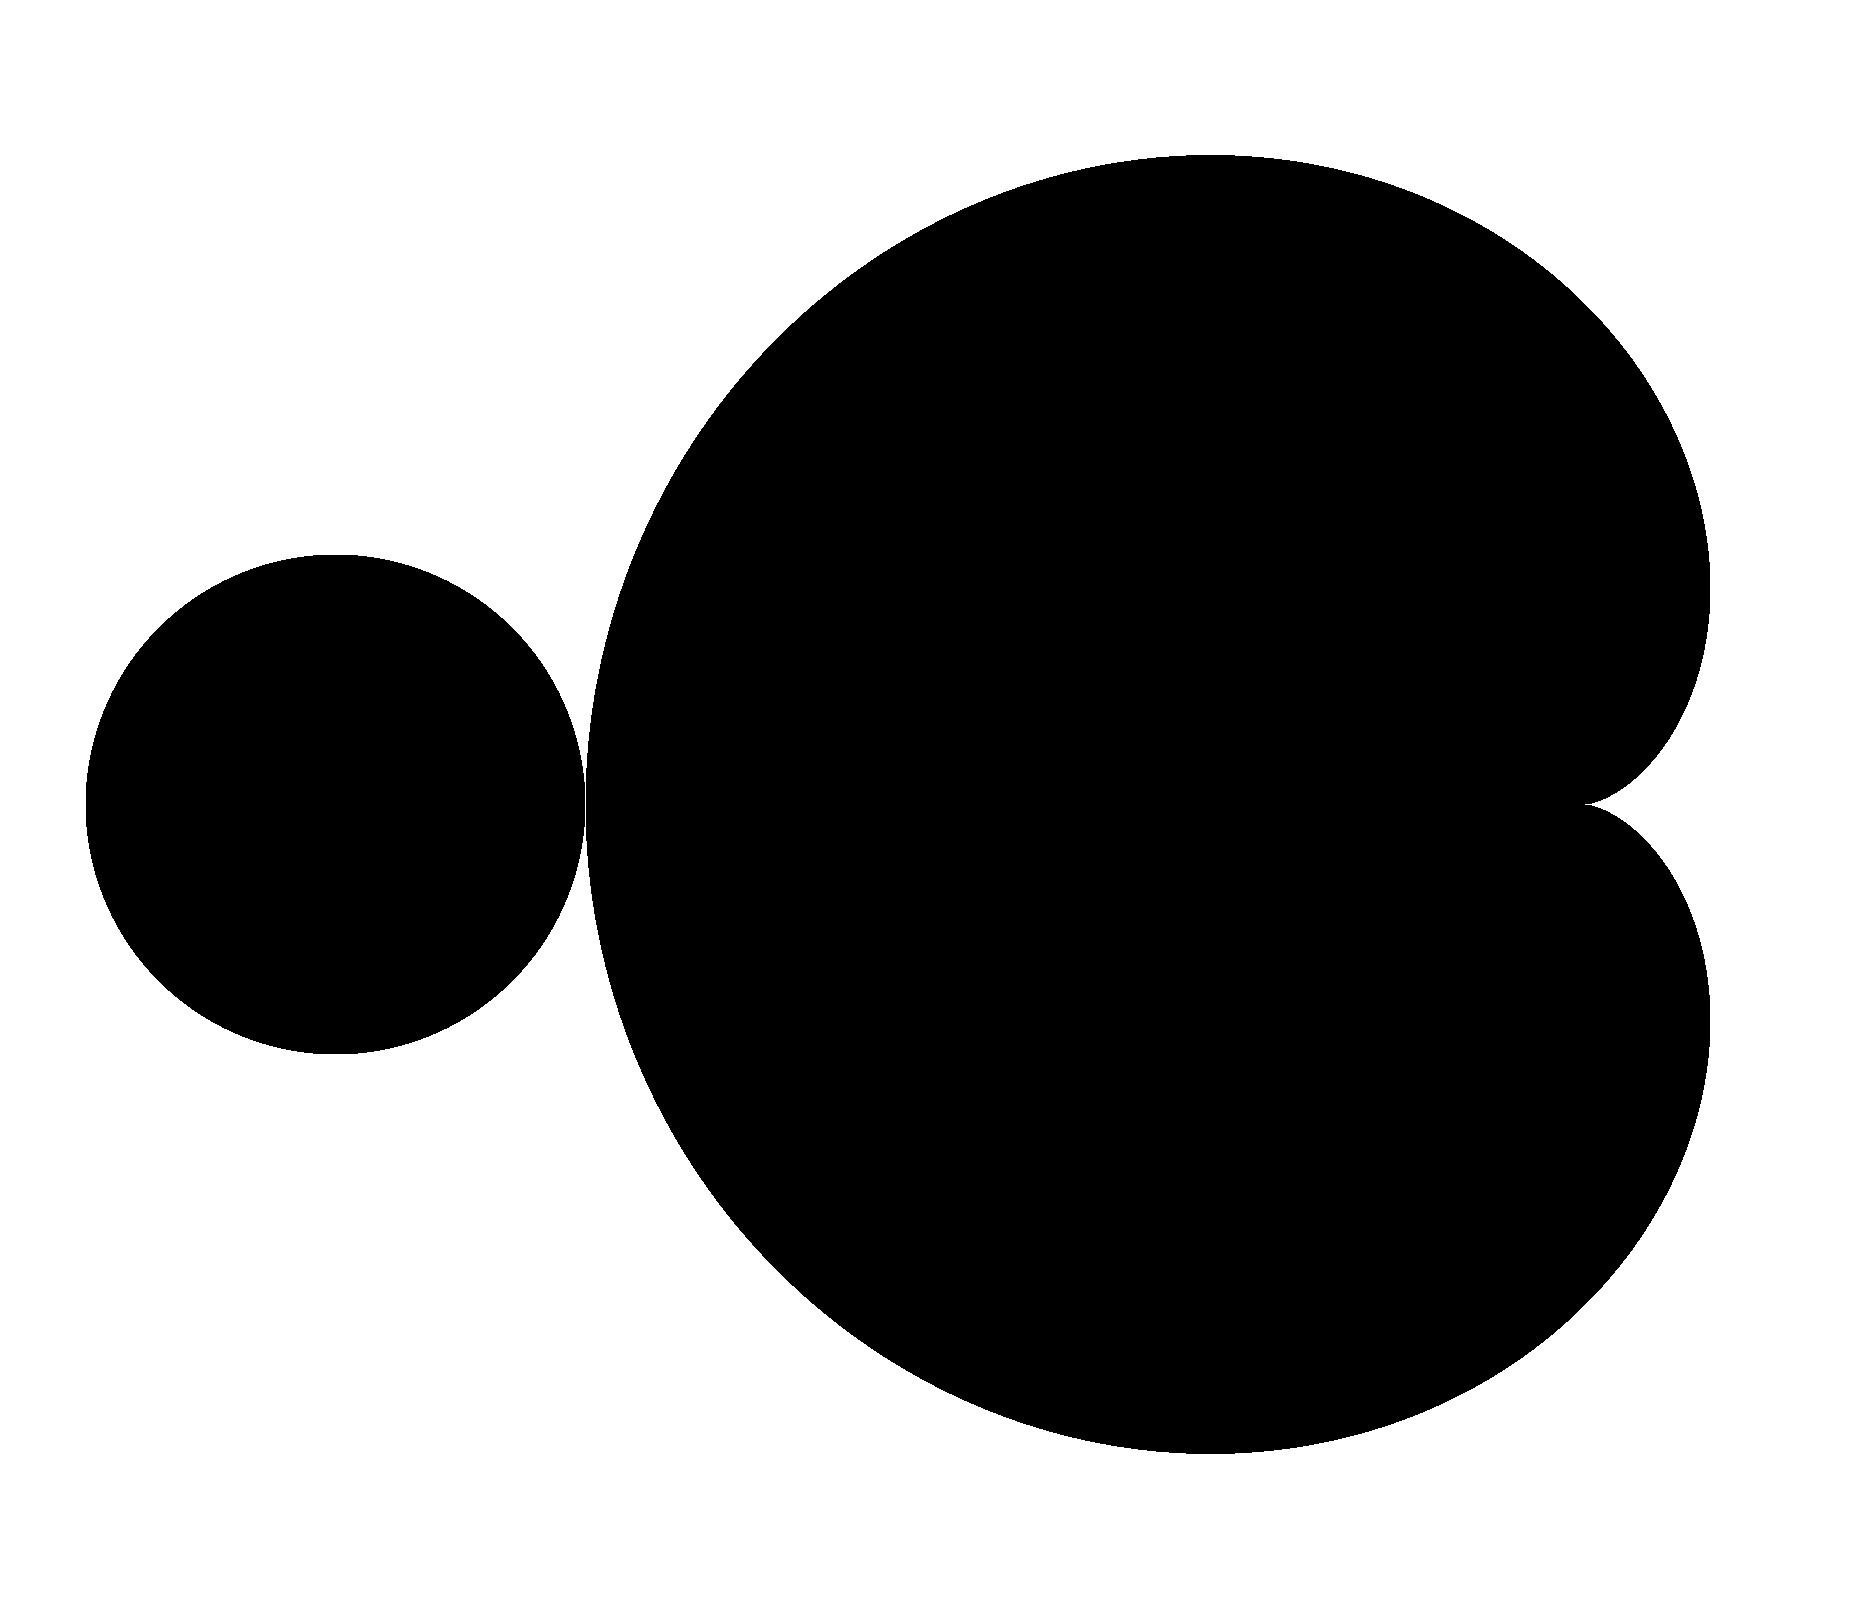
\includegraphics[width=4cm]{graphics/CardioidCircle.png}
\caption{
Kardioida in krog, dobljena s pogojem na točkah $c\in\CC$, 
za katere ima $q_c$ kakšno privlačno fiksno točko ali $2$-cikel.
}
\end{figure}
\noindent Podobno bi lahko naredili tudi z drugimi $2^k$-cikli
za $k\in\N$, a bi morali iskati ničle polinomov višjih stopenj.
\end{primer}



\section{Dinamika v okolici superprivlačnih točk}
V tem razdelku bomo pod drobnogled vzeli fiksne točke, ki so več kot zgolj privlačne. 
To bo pomenilo, da je na okolici teh točk red konvergence vsaj kvadraten. 
Izkazalo se bo, da je dinamika na okolici takih točk ekvivalentna dinamiki preslikave $z\to z^n$ za $n\geq 2$. 
Slednje bo ključno pri obravnavi polinomov, saj imajo ti vedno vsaj eno tako točko $z=\infty$.

\begin{definicija}\label{def:superattractingFixedPoint}
Naj bo dana holomorfna funkcija $f\colon U \to U$. 
Če za fiksno točko $\alpha \in U$ velja $f'(\alpha) = 0$, 
potem $\alpha$ imenujemo {\em superprivlačna fiksna točka} za $f$.
\end{definicija}

\noindent Denimo, da ima holomorfna funkcija $f$ v točki $\alpha$ superprivlačno fiksno točko. 
Tedaj je njen Taylorjev razvoj okoli te točke enak
$$f(z) = \alpha + \sum_{k = n}^\infty a_k (z - \alpha)^k,$$
kje $a_n \neq 0$. 
Število $n \geq 2$ imenujemo {\em lokalna stopnja} superprivlačne fiksne točke.
Pripomnimo, da lahko s konjugacijo $z \to (\alpha - z)$ vsako fiksno točko $\alpha$ premaknemo 
v izhodišče in s tem ohranimo tudi superprivlačnost.
V spodnjih dokazih bomo zato večinkrat predpostavili kar, da je $\alpha=0$.

\subsection{B{\"o}ttcherjeve koordinate}
Kot rečeno se bomo ukvarjali s poenostavitvijo dinamike v okolici superprivlačnih točk.
Pri tem bo ključno orodje vpeljava biholomorfizma, ki mu pravimo tudi B{\"o}ttcherjeve koordinate.
Le ta bo ključen tudi v dokazu povezanosti Mandelbrotove množice.
Podpoglavje je povzeto po \cite[Poglavje~9]{milnor}, kjer bralec lahko poišče še dodatne informacije.

\begin{izrek}[B{\"o}ttcher]\label{izr:Bottcher}
Naj bo $f \colon U \to U$ holomorfna funkcija s superprivlačno fiksno točko $\alpha$.
Tedaj obstajajo $\epsilon>0$, $n\geq 2$, okolica $V\subseteq U$ točke $\alpha$ ter holomorfna in 
konformna preslikava $\phi \colon V \to \D_\varepsilon$ z ničlo v $\alpha$, ki zadošča B{\"o}ttcherjevi enačbi
$$\phi(f(z))=\phi(z)^n,\; z\in V.$$
\end{izrek}

\proof
Brez škode za splošnost lahko predpostavimo, da je $\alpha = 0$. Naša funkcija je torej oblike
$$f(z) = a_nz^n + a_{n+1}z^{n+1} + \cdots \; \text{za } n \geq 2.$$ 
Naj bo $c$ ena izmed rešitev enačbe $c^{n-1}=a_n$. Tedaj velja
\begin{equation*}
\begin{aligned}
cf(z/c) &= a_nc^{-(n-1)}z^n + a_{n+1}c^{-n}z^{n+1} + \dots  \\
&= z^n (1 + a_{n+1}c^{-n}z + \dots) \\
&= z^n (1 + g(z)),
\end{aligned}
\end{equation*}
kjer $g$ holomorfna funkcija, z lastnostjo $g(0) = 0$. 
Ker konjugacija te oblike ne vpliva na rešitve enačbe,
lahko brez škode za splošnost nadaljujemo kar z obravnavo funkcije
$$f(z) = z^n(1 + b_1z + \dots) = z^n(1 + g(z)).$$ 
Sedaj izberimo tak $0 < \varepsilon < 1/2$, 
da za $z \in \D_\varepsilon$ velja $|g(z)|  < \delta$ za nek $0 < \delta < 1/2$, ki ga bomo fiksirali kasneje. 
Iz neenakosti
$$|f(z)| = |z^n||1 + g(z)| < \varepsilon^{n-1} 3/4 < \varepsilon$$
sledi, da je $\D_\varepsilon$ invarianten podprostor za $f$. Seveda je potem invarianten tudi za vse njene iteracije.
Nadalje je s predpisi
\begin{equation*}
\begin{aligned}
\phi_k(z) := (f^k(z))^{n^{-k}} &= (z^{n^k} (1 + n^{k-1}b_1 z + O(z^2)))^{n^{-k}} \\
&= z (1 + c_1z + c_2z^2 + \cdots)
\end{aligned}
\end{equation*}
definirana družina holomorfnih in konformnih preslikav $(\phi_k)_{k\in\N}$, 
ki zadošča  pogoju $\phi_k(f(z)) = \phi_{k+1}(z)^n$.
Naš cilj bo utemeljiti, da ta družina konvergira enakomerno na $\D_\varepsilon$.
V tem primeru je namreč  limitna funckija $\phi$ holomorfna in konformna, zanjo pa bosta bosta veljali tudi željeni enakosti.

Naj bo $\hat{f}(\zeta) := \ln(f(e^\zeta)) =  n\zeta + \ln(1 + g(e^\zeta))$ funkcija, ki je holomorfna na invariantnem podprostoru
$\HH := \exp^{-1}(\D_\varepsilon) = \{x + iy \in \CC \mid x < \varepsilon\}$.
Poiščemo dovolj majhen $\delta$, da velja $|\ln(z)| < 1$ za $|z - 1| < \delta$, iz česar dobimo
$$|\hat{f}(\zeta) - n\zeta| = |\ln(1 + g(e^\zeta))| < 1$$ za $\zeta \in \HH$.
Definiramo še $\hat{\phi}_k(\zeta) := \ln(\phi_k(e^\zeta)) = n^{-k} \hat{f}^k(\zeta)$ in opazimo
$$|\hat{\phi}_{k+1}(\zeta) - \hat{\phi}_k(\zeta)| = n^{-(k+1)}|\hat{f}(\hat{f}^k(\zeta)) - n \hat{f}^k(\zeta)| < n^{-(k+1)}$$
za $\zeta \in\HH$. Ker je $\HH$ vsebovan v levem delu kompleksne ravnine, po Lagrangeovem izreku velja aproksimacija
$|e^z - e^w| < |z - w|$ za vse $\{z, w\} \subset \HH$ in zato
$$|\phi_{k+1}(z) - \phi_k(z)| < |\ln(\phi_{k+1}(z)) - \ln(\phi_k(z))| < n^{-(k+1)}$$ za vse $z \in \D_\varepsilon$.
Torej $(\phi_k)_{k\in\N}$ zadoša {\em Cauchyjevem} pogoju za enakomerno konvergenco na podprostoru $\D_\varepsilon$.
\endproof

V prejšnjem razdelku smo se večinoma ukvarjali z iskanjem konjugacij, ki so nam poenostavile iteracije zahtevnejših preslikav.
Razlog za definicijo B{\"o}ttcherjeve preslikave je enak, saj v okolici superprivlačne fiksne točke
$\phi$ konjugira $f$ v $z \to z^n$.
Vseeno velja opomniti, da so te koordinate za razliko od kojugacij v prejšnjem poglavju definirane zgolj lokalno. 
To pomeni, da z njimi ne moremo opisati dogajanja na celotni sferi $\CCinf$.
Kot pove naslednja trditev, pa jih lahko razširimo na celotno bazo privlačnosti obravnavane superprivlačne točke.

\begin{posledica}\label{pos:expBottcher}
Naj bo $f$ holomorfna in $\alpha$ njena superprivlačna fiksna točka.
Potem lahko B{\"o}ttcherjevo preslikavo $\phi_\varepsilon$ enolično in holomorfno razširimo na $\phi \colon \A_\alpha \to \D$, 
kjer je $\A_\alpha$ baza privlačnosti točke $\alpha$.
\end{posledica}

\proof
Spet lahko predpostavimo, da je $\alpha = 0$ in je zato $\phi_\varepsilon$ definirana na nekem disku $\D_\varepsilon$.
Po definiciji baze privlačnosti je $\lim_{n\to\infty}f^n(z) = 0$ za vsak $z \in \A_\alpha$, torej lahko za vsak $z\in\A_\alpha$ 
najdemo takšen $k\in\N$, da $f^k(z) \in \D_\varepsilon$. Potem lahko definiramo $\phi(z) := \phi_\varepsilon(f^k(z))^{n^{-k}}$,
ki je po lastnosti B{\"o}ttcherjeve preslikave neodvisna od $k\in\N$. 
Iz tega dejstva sledi, da je preslikava $\phi$ dobro definirana tudi na množici $\A_\alpha$.
Kot kompozicija holomorfnih funkcij je tudi holomorfna, 
ker pa je še $\phi_\varepsilon(0) = 0$, velja $|\phi_\varepsilon(f^k(z))| < 1$ za dovolj visoke $k$, 
torej na $\A_\alpha$ velja $|\phi| < 1$.
\endproof

Pripomnimo, da ta razširitev, čeprav holomorfna, ni nujno konformna na $\A_\alpha$, saj je neničeln odvod še vedno
zagotovljen le na neki okolici superprivlačne fiksne točke.
Z gotovostjo pa lahko trdimo, da obstaja lokalni inverz B{\"o}ttcherjeve preslikave $\psi_\varepsilon \colon \D_\varepsilon \to \A_\alpha$, 
za katerega opazimo, da velja $f(\psi_\varepsilon(w)) = \psi_\varepsilon(w^n)$.
V naslednjem izreku bomo obravnavali razširitve takega inverza.

\begin{izrek}\label{izr:invBottcher}
Naj bo $f$ holomorfna preslikava s superprivlačno fiksno točko $\alpha$ in B{\"o}ttcherjevo preslikavo $\phi$.
Za lokalni inverz $\psi_\varepsilon$ obstaja enolična injektivna in konformna razširitev $\psi \colon \D_r \to \A_\alpha$ z maksimalnim radijem $0 < r \leq 1$.
Če je $r = 1$, potem je $\psi \colon \D \to \A_\alpha$ surjekcija, $\alpha$ pa edina kritična točka $f$ na $\A_\alpha$.
Če pa je $r < 1$, potem kritična točka $f$ leži na $\partial(\psi(\D_r)) \subset \A_\alpha$.
\end{izrek}

\proof
Ker je $\phi$ holomorfna in konformna okoli $\alpha$, 
lahko na dovolj majhni okolici $\D_\varepsilon$ definiramo holomorfen in konformen lokalni inverz,
za katerega obstaja analitična razširitev $\psi \colon \D_r \to \A_\alpha$ z maksimalnim radijem $0 < r \leq 1$.
Tedaj za $z\in\D_r$ velja
$$\psi(\{z\}) = f^{-k}(\psi(\{z^{n^k}\})) \subset \A_\alpha,$$
če je število $k\in\N$ dovolj visoko, saj $\psi(w) = \psi_\varepsilon(w) \in \A_\alpha$ za $w$ dovolj blizu $0$.
Zato sledi $\psi(\D_r) \subseteq \A_\alpha$.

Ker za razširitev B{\"o}ttcherjeve preslikave $\phi \colon \A_\alpha \to \D$ iz Posledice \ref{pos:expBottcher} velja, 
da je $\phi(\psi(z)) = z$ za vsak $z\in\D_\varepsilon$, to po analitičnosti $\phi \circ \psi$ drži tudi na $\D_r$.
Torej je $\psi$ injektivna na $\D_r$.
Sedaj utemeljimo še konformnost. 
Denimo, da je $\psi'(w) = 0$ za nek $w\in\D_r$. Potem velja
\begin{equation}\label{psiDer}
\frac{d}{dw} \; (\psi(w^n)) = \frac{d}{dw} \; (f(\psi(w))) = f'(\psi(w)) \psi'(w) = 0,
\end{equation}
torej imamo zaporedje kritičnih točk $(w^{n^k})_{k\in\N}$, ki pa konvergira proti $0$.
Ker je $\psi$ v okolici te točke konformna, pridemo v protislovje.

Če je $r=1$, potem $\psi(\D) \subseteq \A_\alpha$. Recimo, da $\psi(\D) \subsetneq \A_\alpha$, 
torej presek množic $\partial(\psi(\D)) \cap \A_\alpha$ ni prazen. 
Še več, vzemimo točko $z$ iz tega preseka in konstruirajmo zaporedje $(w_k)_k$, za katerega je $\lim_{k\to\infty}\psi(w_k) = z$.
Potem je $$\lim_{k\to\infty}|\phi(\psi(w_k))| = |\phi(z)| = 1,$$ 
saj je $|\phi|$ zvezna na $\A_\alpha$. Ker na $\A_\alpha$ velja $|\phi| < 1$, dobimo protislovje.
Recimo še, da ima $f$ kritično točko v $\beta \in \A_\alpha \smallsetminus \{\alpha\}$. 
Ker je $\psi$ surjekcija v $\A_\alpha$, obstaja $\hat{\beta} \in \D$, da $\psi(\hat{\beta}) = \beta$.
Iz enakosti (\ref{psiDer}) tedaj sledi, da je $\hat{\beta}^n$ kritična za $\psi$, 
kar pa ni mogoče, saj je $\psi$ konformna na $\D$.

Če je $r < 1$, sledi $\overline{\D_{r^n}} \subset \D_r$. 
Ker je $\psi$ homeomorfizem na $\D_r$, velja enakost
$$\overline{\psi(\D_{r^n})} = \psi(\overline{\D_{r^n}})  \subset \psi(\D_r),$$
ker pa je $f$ zvezna, velja še 
$$f(\overline{\psi(\D_r)}) \subset \overline{f(\psi(\D_r))} = 
\overline{\psi(\D_{r^n})} \subset \psi(\D_r) \subset \A_\alpha.$$
Ker iz $x\notin\A_\alpha$ sledi, da je $f(x) \notin \A_\alpha$, 
smo dokazali $\partial(\psi(\D_r)) \subset \overline{\psi(\D_r)} \subset \A_\alpha$.
Izberimo sedaj poljubno točko $w_0 \in \partial(\D_r)$ ter definirajmo $z = \lim_{t\uparrow1} \psi(tw_0)$.
Recimo, da $z \in \partial(\psi(\D_r))$ ni kritična točka za $f$ in zato po izreku o implicitni funkciji 
obstaja lokalni inverz $g$ na neki množici $V_{w_0} \subset \A_\alpha$.
S pogojem $\psi(w) = g(\psi(w^n))$ na $V_{w_0}$ podamo razširitev za $\psi$. 
Če na $\partial(\psi(\D_r))$ ni kritičnih točk, lahko kompakt $\partial(\D_r)$ pokrijemo z 
zaporedjem $V_w$ za $w \in \partial(\D_r)$ ter tako dobimo razširitev $\psi$ na $\D_m$ za $r < m \leq 1$.
Ker je $r$ maksimalni radij, smo prišli v protislovje.
\endproof

\subsection{Superprivlačna točka $\infty$}
V nadaljevanju diplome lokalne teorije superprivlačnih točk ne bomo uporabljali v vsej splošnosti. 
Zato se bomo v tem razdelku osredotočili na polinome stopnje $d\geq 2$.
Vsak tak polinom ima namreč superprivlačno točko $z=\infty$,  kar bomo dokazali z naslednjo trditvijo.

\begin{trditev}
Naj bo $p$ polinom stopnje $d\geq2$. 
Tedaj je $z=\infty$ njegova superprivlačna fiksna točka.
\end{trditev}

\proof
Na razširjeni kompleksni ravnini definirajmo $h \colon z \to 1/z$ in s to preslikavo $p$ konjugiran par 
$q := h \circ p \circ h^{-1}$. Opazimo, da za vodilni koeficient $a_d$ polinoma $p$ velja
$$\lim_{z\to0} q(z) / z^d = \lim_{\zeta\to\infty} \zeta^d / p(\zeta) = a_d.$$
Sledi, da je $q(0) = q^{(1)}(0) = \cdots = q^{(d-1)}(0) = 0$ in $q^{(d)}(0) \neq 0$,
kar pomeni, da ima $q$ v izhodišču superprivlačno fiksno točko z lokalno stopnjo $d$.
\endproof

\begin{opomba}\label{op:conjCriticalP}
Če odvajamo $q$, dobimo
$$q'(z) = \frac{p'(1/z)}{(zp(1/z))^2}.$$
Iz tega sledi, da so poleg $0$ edine možne kritične točke za $q$ 
enake tistim točkam $\zeta$, za katere je $1/\zeta$ kritična točka polinoma $p$.
\end{opomba}

Vidimo torej, da je $\infty$ superprivlačna fiksna točka vsakega polinoma stopnje $d\geq 2$ in 
da je njena lokalna stopnja enaka $d$.
Naslednja trditev pa nam pove, da so v njeni bazi privlačnosti vsa kompleksna števila, 
ki imajo dovolj veliko absolutno vrednost.

\begin{trditev}\label{trd:escaperadius}
Naj bo dan kompleksni polinom oblike
$$p(z) = a_{d} z^{d} + a_{d-1} z^{d-1} + \dots a_1 z + a_0,$$
kjer $d\geq 2$ in $a_d \neq 0$.
Če za $C = \sum_{i = 0}^{d-1}|a_i|$ in $\lambda > 1$ velja
$$|z| \geq \max\left\{1, 2C / |a_d|, \left(2\lambda / |a_d|\right)^{\frac{1}{d -  1}}\right\},$$ 
potem je $|p(z)| \geq \lambda |z|.$
\end{trditev}

\proof
Naredimo lahko naslednjo oceno:
\begin{align*}
|p(z)| &= |a_d z^d + a_{d-1} z^{d-1} + \dots + a_1 z + a_0|   \\
&\geq |a_d z^d| - |a_{d-1} z^{d-1} + \dots + a_1 z + a_0|  \\
&\geq |a_d z^d| - (|a_{d-1}z^{d-1}| + \dots + |a_1 z| + |a_0|)  \\
&\geq |a_d z^d| - |z^{d-1}|\left(|a_{d-1}|+ \dots + |a_1| + |a_0|\right) \\
&\geq |z^d| |a_d| / 2 \\ 
&\geq \lambda |z|.
\end{align*}
V prvi in drugi neenakosti smo uporabili trikotniško neenakost,
pri tretji je bil upoštevan pogoj $|z| \geq 1$, 
v četrti pa dejstvo, da je $2C \leq |a_d z|$.
V zadnji neenakosti je bila uporabljena ocena $|a_dz^{d-1}| \geq 2\lambda$.
\endproof

\begin{primer}
Z uporabo Trditve \ref{trd:escaperadius} na preslikavi $z \to z^2$ 
dobimo za nek $\lambda>1$ radij $\max\{1, 0, 2\lambda\} = 2\lambda$.
Torej nam trditev pove, da je konvergenca iteracij preslikave $z \to z^2$ proti točki $\infty$ zagotovljena na $\CC \smallsetminus \overline{\D_2}$.
Opazimo, da ta radij ni optimalen, saj velja 
$$\lim_{k\to\infty} z^{2^k} = \infty$$
že za vse $z$ na $\CC \smallsetminus \overline{\D}$. 
\end{primer}
\vskip 2mm

Kot je razvidno iz zgornjih postopkov, 
pri analizi točke $z=\infty$ praviloma vedno vpeljemo recipročno konjugacijo,
ki omogoča, da namesto neskončnosti obravnavamo izhodišče. 
V tem kontekstu bomo nekoliko prilagodili tudi B{\"o}ttcherjeve koordinate.

\begin{definicija}\label{def:invertedBottcherMap}
Naj bo dan polinom $p$ stopnje $d\geq2$ in naj bo $q$ funkcija, dobljena s konjugiranjem $p$ s konjugacijo $z \to 1/z$.
Ta ima v $0$ superprivlačno fiksno točko stopnje $d$ in pridruženo B{\"o}ttcherjevo preslikavo $\hat{\phi} \colon \A_0 \to \D$,
podano s predpisom $$\hat{\phi}(z) = \lim_{n\to\infty}(q^n(z))^{d^{-n}}.$$
Če konjugiramo z recipročno konjugacijo še $\hat{\phi}$, dobimo na neki okolici $\infty$ tako imenovano {\em invertirano B{\"o}ttcherjevo preslikavo}
$\phi \colon \A_\infty \to \CCinf\smallsetminus\overline{\D}$, ki jo torej definiramo s predpisom
$$\phi(z) := (\hat{\phi}(z^{-1}))^{-1} = \lim_{n\to\infty}(p^n(z))^{d^{-n}}.$$
\end{definicija}

Na ta način smo za vsak polinom stopnje $d\geq 2$ na nov in bolj sugestiven način definirali B{\"o}ttcherjevo preslikavo, 
ki pa se ujema s tisto iz predhodnega razdelka.

\begin{primer}
Za preslikavo $z\to z^d$ dobimo
$$\phi_k(z) =  \left(\left(z \to z^d\right)^k(z)\right)^{d^{-k}} = z,$$
torej je njena invertirana B{\"o}ttcherjeva preslikava enaka identiteti na $\CCinf\smallsetminus\overline{\D}$.
To je očitno, saj je preslikava že v obliki, v katero bi jo sicer želeli konjugirati.
\end{primer}

\begin{opomba}
V kontekstu Definicije \ref{def:invertedBottcherMap} lahko bazo privlačnosti $\A_0$ eksplicitno zapišemo kot
$$\A_0 = \{1/z \in \CC \mid \lim_{k\to\infty}p^k(z) = \infty\}.$$
Z raziskovanjem množic te oblike se bomo ukvarjali v naslednjem poglavju.
\end{opomba}




\section{Juliajeva in Mandelbrotova množica}
Leta 1917 sta francoska matematika {\em Gaston Julia} in {\em Pierre Fatou} neodvisno naznanila
rezultate o iteraciji kompleksnih racionalnih funkcij ene spremenljivke.
V letih, ki so sledila, so ti postavili temelje za vejo matematike, ki jo danes imenujemo kompleksna dinamika.
Po preučevanju rezultatov francoskih matematikov je teorijo znova populariziral {\em Benoit Mandelbrot}, 
ko je leta 1975 skoval besedo {\em fraktal}.
Ta opisuje lastnost množic, ki obdržijo grobo in kompleksno strukturo na poljubni bližini, primer česar je samopodobnost.
Z njegovim delom na računalniškem področju so te množice prišle v svet umetnosti, 
našle pa tudi uporabo v modeliranju narave, ki pogosto izraža fraktalične oblike.
V poglavju si bomo takšne množice ogledali.
Osredotočili se bomo na polinomske funkcije in večinoma obravnavali 
{\em Douady-Hubbardovo družino kvadratnih polinomov} $\QQ := \{q_c \colon z \to z^2 + c \mid c \in \CC\}$.
Kot smo dokazali v drugem poglavju, ta družina do konjugacije natančno pooseblja dinamiko vseh kvadratnih polinomov.

\subsection{Juliajeve množice}
Eden izmed glavnih dosežkov matematika Gastona Juliaja je karakterizacija množice, ki je dobila ime po njem.
Množica je sicer že tonila v pozabo, dokler ni teorije obudil Benoit Mandelbrot.
Čeprav je ta teorija v splošnem širša in opisana za večji razred funkcij, jo bomo mi obravnavali le za polinome.
Vseeno pa se bo izkazalo, da kljub preprostejši definiciji in polinomskemu tipu dinamike taka množica ne bo izgubila svoje kompleksne, 
fraktalne oblike. Podpoglavje je povzeto po \cite[Poglavje~9]{milnor}, kjer lahko bralec najde še dodatna pojasnila in teorijo.

\begin{definicija} \label {def:Julia}
Naj bo $p \: \colon \CC \to \CC$ polinom stopnje $d\geq2$. 
{\em Napolnjena Juliajeva množica} za $p$ je definirana kot 
$$\J_p^\ast := \{z_0 \in \CC \: | \: \text{orbita $z_0$ je omejena}\}.$$
{\em Juliajevo množico} $\J_p$ definiramo kot rob napolnjene Juliajeve množice,
njen komplement pa imenujemo {\em Fatoujeva množica}.
\end{definicija}

\begin{opomba}
Juliajeva in Fatoujeva množica določata dve vrsti obnašanja za pripadajoči polinom.
In sicer, na Fatoujevi množici je obnašanje orbit predvidljivo, medtem, ko je na Juliajevi to obnašanje kaotično.
To pomeni, da poljubno majhne spremembe v izbiri začetne točke na Juliajevi množici
močno vplivajo na obnašanje njene orbite.
\end{opomba}

\noindent Pripomnimo, da je za polinom stopnje $d\geq2$ napolnjena Juliajeva množica komplement baze privlačnosti
superprivlačne fiksne točke $\infty$. 
Ker pa so polinomi zvezni, po Opombi \ref{op:attBasinOpen} vidimo, da je napolnjena Juliajeva množica zaprta. 
Zato vsaka napolnjena Juliajeva množica vsebuje svojo Juliajevo množico.
Če se spomnimo še Trditve \ref{trd:escaperadius}, sledi ob tem celo kompaktnost obeh množic v kompleksni ravnini.

\begin{figure}[h]
\includegraphics[width=6cm]{graphics/douadyRabbitGray.png}
\caption{
Napolnjena Juliajeva množica polinoma $q_{(-0.123+0.745i)}$ družine $\QQ$,
poimenovana {\em Douadyjev zajec} po francoskem matematiku {\em Adrienu Douadyju}.
}
\label{img:DouadyRabbit}
\end{figure}

\begin{primer}
Oglejmo si dinamiko preslikave $q_0$ na njeni Juliajevi množici.
V Primeru \ref{primer:QuadTranslation} smo že ugotovili, da orbite na $\D$
konvergirajo proti izhodišču ter na $\CC \smallsetminus \overline{\D}$ k $\infty$.
Ker $q_0$  krožnico $\SSS$ preslika vase, sledi, da je 
$$\J_{q_0}^\ast = \overline{\D} \quad \text{in} \quad \J_{q_0} = \SSS.$$

Vzemimo točko $a\in\SSS$ in jo izrazimo v polarnih koordinatah kot $e^{2\pi i \theta_a}$.
Preslikavo $q_0$ lahko lažje opišemo na $\SSS$ s pomočjo preslikave $\iota \colon [0, 1) \to [0, 1)$,
ki je definirana v dvojiškem sistemu kot levi zamik zaporedja
$$\iota(\theta_a) = \iota((0.a_1 a_2 a_3\dots)_2) := (0.a_2a_3a_4\dots)_2.$$
Opazimo, da za $k\in\N$ velja 
$$q_0^k(a) = \exp(2\pi i \iota^k(\theta_a)).$$
Ločimo dva primera glede na zapis števila $\theta_a$,
\begin{itemize}
\item[(1)] $\theta_a$ se v dvojiškem sistemu da zapisati s končno mnogimi decimalkami,
\item[(2)] $\theta_a$ se v dvojiškem sistemu ne da zapisati s končno mnogimi decimalkami.
\end{itemize}
V prvem primeru za nek $k\in\N$ velja 
$$\theta_a = (0.a_1a_2\dots a_k)_2 \implies \iota^k(\theta_a) = 0 \implies q_0^k(a) = 1.$$
Tako vidimo, da je dinamika  od $k$ naprej opisana z mirovanjem orbite na fiksni točki $1$.
V drugem primeru pa po Posledici \ref{pos:odbojnaKonv} konvergence k fiksni točki ne bo, saj je ta odbojna. 
Za primer (2) ločimo še dva podprimera
\begin{itemize}
\item[(2.1)] $\theta_a$ je racionalno število,
\item[(2.2)] $\theta_a$ je iracionalno število.
\end{itemize}
Ker so v binarnem zapisu racionalnih števil zaporedja števk od nekje naprej periodična,
sledi, da bodo orbite od nekje naprej opisane s cikli.
V drugem primeru pa se iz dokaza Leme \ref{lema:Jacobi} spomnimo, da se točke v orbiti ne ponavljajo,
zato ciklov ne bo. Primer pa ni povsem enak kot v lemi, saj za iracionalno število 
$$\theta_a = (0.101001000100001\dots)_2$$
velja, da ima orbita stekališča le pod koti oblike $2^{-k}$ za $k\in\N_0$, torej ni gosta na $\SSS$.
Po drugi strani pa lahko z zaporednim naštevanjem vseh končnih zaporedij ničel in enic konstruiramo 
iracionalno število $\theta_a$, katerega orbita je gosta na $\SSS$.

Vidimo, da se dinamika na $\SSS$ za števila, ki so si poljubno blizu, močno razlikuje.
Ta lastnost je osnova za karakterizacijo Juliajevih množic splošnih funkcij.
\end{primer}

\begin{izrek}[Osnovna dihotomija]\label{izr:FundamentalDichotomy}
Za polinom $p$ stopnje $d\geq2$ je $\J_p$ povezana natanko tedaj, ko $\J^\ast_p$ vsebuje vse kritične točke $p$.
Če kritična točka leži izven $\J_p^\ast$, potem ima $\J_p$ neštevno mnogo komponent.
\end{izrek}

\proof
V nadaljevanju diplomskega dela bomo potrebovali le prvi del trditve,
zato se bomo omejili le na njegov dokaz.
Dokaz drugega dela lahko bralec poišče v viru \cite[Stran~99-100]{milnor}.

Recimo najprej, da $\J_p^\ast$ vsebuje vse kritične točke $p$.
Definirajmo $\zeta \colon z \to 1/z$ in $q := \zeta \circ p \circ \zeta^{-1}$ konjugiran par za $p$.
Za $q$ naj bo $\phi_q \colon A \to \D$ razširjena B{\"o}ttcherjeva preslikava,
definirana na $A := \zeta(\CCinf \smallsetminus \J_p^\ast)$ okolici superprivlačne fiksne točke v izhodišču.
Opazimo, da je po predpostavki in Opombi \ref{op:conjCriticalP} to edina kritična točka za $q$ v množici $A$.
Po Izreku \ref{izr:invBottcher} zato obstaja biholomorfna razširitev lokalnega inverza B{\"o}ttcherjeve preslikave, 
$\psi_q \colon \D \to A$. Definirajmo potem biholomorfno preslikavo
$$\left(\psi := \zeta \circ \psi_q \circ \zeta^{-1} \right) \colon \CCinf \smallsetminus \overline{\D} \to \CCinf \smallsetminus \J_p^\ast$$
in zaporedje kolobarjev
$$K_n := \{w \in \CC \mid 1 < |w| < 1 + 1/n\}.$$
Ker je $\psi$ homeomorfizem, se kolobarji okoli $\overline{\D}$ preslikajo v topološke kolobarje okoli $\J_p^\ast$, 
iz česar pa po zveznosti $\psi$ sledi
$$\J_p = \bigcap_{n\in\N} \overline{\psi\left(K_n\right)}.$$
Ker so $K_n$ povezane, so po zveznosti $\psi$ povezane $\psi(K_n)$,
seveda pa so povezana potem tudi zaprtja teh množic.
Iz tega sledi, da je
$$\overline{\psi\left(K_1\right)} \supseteq \overline{\psi\left(K_2\right)} 
\supseteq \overline{\psi\left(K_3\right)} \supseteq \cdots$$
zaporedje padajočih povezanih kompaktov v Hausdorffovem prostoru, zato je povezan tudi njihov presek.
Omenimo še, da je tudi napolnjena Juliajeva množica povezana, 
saj je $\psi(\CCinf \smallsetminus \overline{\D}) = \CCinf \smallsetminus \J_{p}^\ast$ enostavno povezana.

Recimo sedaj, da kritična točka za $p$ leži izven $\J_p^\ast$. 
Naj bo spet $\phi$ invertirana B{\"o}ttcherjeva preslikava. 
S pomočjo Izreka \ref{izr:invBottcher} lahko na enak način kot v dokazu implikacije v desno
sedaj za nek najmanjši $r > 1$ konstruiramo biholomorfizem
$$\psi \colon \CC \smallsetminus \overline{\D_r} \to U \subset \overline{U} \subset \CC \smallsetminus \J_p^\ast.$$
Izrek nam pove tudi, da kritična točka $z_0$ leži na robu $U$. Za $z_1 = p(z_0)$ potem velja 
$$|\phi(z_1)| = |\phi(p(z_0))| = r^d > r,$$
torej je $z_1 \in U$.
Definirajmo žarka
$$C := \{t \cdot \phi(z_1) \mid t \geq 1\} \subset \CC \smallsetminus \D_{r^d} \quad \text{in} \quad R := \psi(C) \subset U.$$
Potem velja
$$Q := p^{-1}(R) = p^{-1}(\psi(C)) = \psi(\sqrt[d]{C}) \subset \overline{U},$$
saj je $|\phi(z_1)t| \geq r^d$ za vsak $t \geq 1$.
Torej množica $Q$ vsebuje $d$ vej, asociiranih z $\sqrt[d]{C}$.
Ker ima enačba $p(z) = z_1$ v kritični točki $z_0$ rešitev druge stopnje, sledi, da $(z - z_0)^2$ deli $p(z) - z_1$,
torej obstajata v $Q$ vsaj dve veji z začetkom v $z_0$, ki ju označimo z $Q_1$ in $Q_2$.
Ker je $\psi$ injekcija v vseh točkah $\sqrt[d]{C}$ razen v teh na $\SSS_r$, 
sledi, da se ti veji ne sekata nikjer drugje razen v $z_0$.
Torej za neki odprti množici $V_1$ in $V_2$ velja
$$V_1 \cup V_2 = \CC \smallsetminus (Q_1 \cup Q_2).$$
Dokazati želimo, da je $\partial(p(V_j)) \subseteq R$ za $j =1, 2$.
Če je $a \in \partial(p(V_j))$, potem obstaja zaporedje $(a_n)_n$, za katerega velja $p(a_n) \to a$.
Izberimo konvergentno podzaporedje $(a_{n_k})_k$ z limito $\tilde{a}$ in opazimo, 
da iz tega, da je $p(\tilde{a}) = a \in \partial(p(V_j))$, sledi $\tilde{a} \notin V_j$, saj je $p(V_j)$ odprta po izreku o odprti preslikavi.
Potem pa je 
$$\tilde{a} \in \partial V_j = Q_1 \cup Q_2 \implies a = p(\tilde{a}) \in p(Q_1 \cup Q_2) = R.$$
Ker je $\CC \smallsetminus R$ povezana, sledi $p(V_j) \supseteq \CC \smallsetminus R \supseteq \J_p^\ast,$
saj je $R \subset U$. Množici
$$J_1 := \J_p \cap V_1 \quad \text{in} \quad J_2 := \J_p \cap V_2$$
sta potem disjunktni in zanju velja $J_1 \cup J_2 = \J_p$.
To je posledica tega, da je
$$\J_p \subseteq \J_p^\ast \implies \J_p \cap Q = \emptyset \implies \J_p \subset V_1 \cup V_2.$$
Ker pa iz $p(V_j) \supseteq \J_p^\ast$ sledi $p(J_1) = p(J_2) = \J_p,$ velja tudi $\J_p^\ast \cap V_j \neq \emptyset$ in zato
smo za $\J_p$ dobili odprto, neprazno ločitev $(V_1, V_2)$.
\endproof

\begin{primer}
Poskusimo poiskati tudi Juliajevo množico za preslikavo $q_{-2}$.
To bomo naredili s pomočjo konjugacije med $q_0$ in $q_{-2}$. 
Trdimo, da je $h \colon z \to z + z^{-1}$
konjugacija med dinamičnima sistemoma $(q_0, U)$ in $(q_{-2}, V)$, kjer
$$U := \CC \smallsetminus \overline{\D} \quad \text{in} \quad V := \CC \smallsetminus \overline{\I_2}$$
za odprt, simetričen, realni interval $\I_2 := (-2, 2)$.
Iz tega bo sledilo, da $U$ ne seka napolnjene Juliajeve množice za $q_{-2}$.

Vzemimo $\zeta \in V$ in rešimo enačbo $h(z) = z + z^{-1} = \zeta .$
Dobimo dve rešitvi
$$z_{1, 2} = \frac{\zeta \pm \sqrt{\zeta^2 - 4}}{2}.$$
Opazimo da je produkt teh rešitev enak $1$. 
To pomeni, da bodisi obe rešitvi ležita na enotski krožnici $\SSS$ bodisi je ena znotraj, druga pa zunaj nje. 
Prvi primer vodi v protislovje, saj iz enakosti $z = e^{i\theta}$ sledi 
$$\zeta = e^{i\theta} + e^{-i\theta} = 2\cos(\theta) \in \overline{\I_2},$$
torej $\zeta \notin V$. 
Zato je edini možen primer drugi, ko ena rešitev leži v $U$, druga pa v $\CC \smallsetminus U$.
Iz tega sledi, da ima enačba v $U$ natanko eno rešitev, kar pa pomeni, da je $h$ bijekcija iz $U$ v $V$.
Nadalje velja 
$$h(q_0(z)) = z^2 + z^{-2} = (z - z^{-1})^2 - 2 = q_{-2}(h(z)).$$
Ker je $h$ še konformna na $U$, je po izreku o implicitni funkciji holomorfen tudi inverz.

Ostane nam še vprašanje dinamike $q_{-2}$ na realnem intervalu $\overline{\I_2}$.
Ker je $z=2$ fiksna točka za $q_{-2}$ in je 
$q^2_{-2}(0) = q_{-2}(-2) = 2,$
sledi $\{0, -2, 2\} \subset \J_{q_{-2}}^\ast.$
To je v resnici vse, kar potrebujemo, da utemeljimo
$$\J_{q_{-2}} = \J^\ast_{q_{-2}} = \overline{\I_2}.$$
Razlog za to je Osnovna dihotomija, saj napolnjena Juliajeva množica za $q_{-2}$ vsebuje njeno edino kritično točko v izhodišču,
torej je povezana. Ker pa vsebuje še točki $z = \pm 2$, sledi, da je enaka $\overline{\I_2}$.
\end{primer}



\subsection{Mandelbrotova množica}
Poljski matematik {\em Benoit Mandelbrot} je, po raziskovanju fraktalnih oblik, leta 1980 populariziral 
{\em Mandelbrotovo množico} in jo z njeno izjemno kompleksno obliko,
a enostavno definicijo, uveljavil kot eno najzanimivejših množic v matematiki.
Leta 1982 so rezultati francoskih matematikov {\em Adriena Douadyja} in njegovega bivšega študenta {\em Johna Hubbarda}
podali mnogo globokih karakteristik topologije Mandelbrotove množice, med katerimi je pomembnejša njena povezanosti.
Predstavitev njunega dokaza je glavni cilj tega podpoglavja. 
Pred tem se spomnimo družine preslikav $q_c \colon z \to z^2 + c$, katerih pomembnost smo utemeljili v Trditvi \ref{trd:quadraticConjugation}.
Zaradi enostavnosti za $n\in\N_0$ označimo $c_n := q_c^n(0)$.

\begin{definicija} \label {def:Mandelbrot}
Družino
$$\M := \{c \in \CC \mid  (c_n)_n \; \text{ je omejeno zaporedje}\}$$
imenujemo {\em Mandelbrotova množica}.
\end{definicija}

\noindent S tako enostavno definicijo je podana topološko zelo kompleksna množica.
Japonski matematik {\em Mitsuhiro Shishikura} je leta 1998 celo dokazal,
da ima njen rob {\em Hausdorffovo dimenzijo} enako $2$.
Bralec lahko več informacij poišče v viru \cite{shishikura}.

\begin{figure}[h]

\includegraphics[width=6cm]{graphics/mandelbrot_plain.png}
\caption{Mandelbrotova množica.}
\label{img:mandelbrotPlain}
\end{figure}

Iz slike je razvidna simetrija Mandelbrotove množice glede na realno os.
To je posledica tega, da je $\overline{c}_n = \overline{c_n}$ za vsak $(n, c) \in \N_0\times\CC$.
Res, za $c\in\CC$ velja $\overline{c}_0 = \overline{c_0}$ in
$$\overline{c}_{n+1} = \overline{c}_n^2 + \overline{c} = 
\overline{c_n}^2 + \overline{c} = \overline{c_n^2} + \overline{c} = \overline{c_n^2 + c} = \overline{c_{n+1}},$$
torej dobimo dokaz z načelom indukcije.

\begin{opomba}\label{op:MandelbrotMotivation}
Iz Definicije \ref{def:Julia} sledi
$$\M = \{c \in \CC \mid 0 \in \J_{q_c}^\ast\}.$$
Ker pa je izhodišče edina kritična točka polinomov $q_c$ za $c\in\CC$, je
po Izreku \ref{izr:FundamentalDichotomy} Mandelbrotova množica
družina točk $c$, za katere ima $q_c$ povezano Juliajevo množico.
\end{opomba}

\begin{primer}
V Primeru \ref{primer:QuadFixCyc} smo opisali $c \in \CC$, 
za katere imajo $q_c$ privlačno fiksno točko ali privlačni $2$-cikel.
{\em Pierre Fatou} je dokazal, da baza privlačnosti vključuje kritično točko $0$,
iz česar sledi, da dobljene točke ležijo v Mandelbrotovi množici.
Izrek, skupaj z dokazom, je naveden v viru \cite[Izrek~8.6]{milnor}.

\begin{figure}[h]

\includegraphics[width=6cm]{graphics/mand.png}
\caption{Kardioida in krog znotraj Mandelbrotove množice.}
\end{figure}

\noindent Kot bi morda lahko sklepali iz slike, se izkaže celo, 
da rob omenjenih množic leži na robu Mandelbrotove množice.
\end{primer}

\begin{trditev}\label{trd:MandelbrotBounded}
Velja $\M = \{c \in \CC \mid \{c_n\}_n \subset \overline{\D_2} \}.$
\end{trditev}

\proof
Fiksirajmo $c \in \CC$ in definirajmo
$$W_c = \{z \in \CC \mid |z| > 2 \; \text{in} \; |z| \geq |c|\}.$$
Naj bo $c_n \in W_c$ za neki $n \in \N$ in $1 < \lambda < |c_n| - 1$. Potem velja
$$|c_{n+1}| = |c_n^2 + c| \geq |c_n|^2 - |c| \geq |c_n|^2 - |c_n| = |c_n| (|c_n| - 1) > \lambda|c_n|,$$
kar pomeni, da je $c_{n + 1} \in W_c$. 
Če induktivno nadaljujemo, ugotovimo, da velja 
$$\lim_{m \to \infty}c_{n + m} = \infty.$$
Za $c \in \M$ zato sledi, da množica
$$\CC \smallsetminus W_c = \{z \in \CC \mid |z| \leq 2 \; \text{ali} \; |z| < |c|\}$$
vsebuje zaporedje  $(c_n)_n$. Ker pa potem vsebuje tudi $c = c_1$, 
velja še $|c| \leq 2$.
\endproof

Če za $(n,c) \in \N_0 \times \CC$ definiramo $p_n \colon \CC \to \CC$ s predpisom  $ p_n(c) = c_n$, 
dobimo polinomsko in zato zvezno funkcijo v odvisnosti od $c$.
Zgornja trditev nam tako omogoča zapisati 
$$\M = \bigcap_{n \in \N} p_n^{-1}\left(\overline{\D_2}\right).$$
Tako vidimo, da je $\M$ kompaktna podmnožica $\CC$.
Naslednji izrek, ki ga bomo dokazali s serijo pomožnih trditev, pa bo povedal, 
da je Mandelbrotova množica kljub nenavadni obliki tudi povezana.
Dokaz bo sledil viru \cite[Izrek~5.3]{stoll}.

\begin{izrek}[Douady-Hubbard]\label{izr:DouadyHubbard}
Mandelbrotova množica je povezana.
\end{izrek}

\proof
Najprej opazimo, da iz $c = c_1$ sledi, da je 
$$\M = \{c \in \CC \mid c \in \J_{q_c}^\ast\}.$$
S tem v mislih definirajmo preslikavo, na kateri bo temeljil dokaz.

\begin{definicija}\label{def:MandelBottcher}
Naj bo $\phi_c \colon \CC \smallsetminus \J_{q_c}^\ast \to \CC \smallsetminus \overline{\D}$
invertirana B{\"o}ttcherjeva preslikava za $q_c$.
{\em Mandelbrot-B{\"o}ttcherjevo preslikavo} 
$\Phi \colon \CCinf \smallsetminus \M \to \CCinf \smallsetminus \overline{\D}$ 
definiramo s predpisoma
$$\Phi(c) := \phi_c(c) \quad \text{in} \quad \Phi(\infty) := \infty.$$
\end{definicija}

V nadaljevanju bo naš edini cilj dokazati, da je preslikava $\Phi$ homeomorfizem,
kar pa bo posledica sledečih pomožnih trditev.

\begin{lema}\label{lem:holMandelBottcher}
Preslikava $\Phi$ je holomorfna na $\CCinf \smallsetminus  \M$.
\end{lema}

\proof
Za $\phi_c^{(k)}(z) = (q_c^k(z))^{2^{-k}}$ definiramo
$$\phi_c(z) := \lim_{k\to\infty}\phi_c^{(k)} (z) = z\prod_{k=0}^\infty \frac{\phi_c^{(k+1)}(z)}{\phi_c^{(k)}(z)}.$$
Ker so $(c, z) \to \phi_c^{(k)}(z)$ za $k\in\N_0$ holomorfne, 
bo produkt v primeru enakomerne konvergence na nekem območju tam holomorfen tudi sam.
Pri enakomerni konvergenci si lahko pomagamo z {\em Weierstrassovim kriterijem}, saj velja
$$
\ln\left(\left|\frac{\phi_c^{(k+1)}(z)}{\phi_c^{(k)}(z)}\right|\right) 
= \ln\left(\left|\frac{(q_c^{k+1}(z))^{2^{-(k+1)}}}{(q_c^{k}(z))^{2^{-k}}}\right|\right) 
= 2^{-(k+1)} \ln\left(\left|1 + \frac{c}{(q_c^k(z))^2}\right|\right)
\leq 2^{-(k+1)}.
$$
To pomeni, da je
$$
\ln\left(\left|\frac{\phi_c(z)}{z}\right|\right)
= \ln\left(\left|\prod_{k=0}^\infty \frac{\phi_c^{(k+1)}(z)}{\phi_c^{(k)}(z)}\right|\right)
= \sum_{k=0}^\infty\ln\left(\left|\frac{\phi_c^{(k+1)}(z)}{\phi_c^{(k)}(z)}\right|\right) 
\leq \sum_{k=0}^\infty 2^{-(k+1)} = 1
$$ 
za vse $(c, z)$, kjer $|z| > m$ za dovolj velik $m > 0$ ter $|c| < \varepsilon$ za dovolj majhen $\varepsilon > 0$.
Zato je $(c, z) \to \phi_c(z)/z$ holomorfna na tem območju, posledično pa je to res tudi za $(c, z) \to \phi_c(z)$.
Podobno kot v dokazu Posledice \ref{pos:expBottcher} lahko za to preslikavo definiramo holomorfno razširitev na
$$\E := \{(c, z) \mid z \notin \J_{q_c}^\ast\} \supset \{(c, c) \mid c\in \CC \smallsetminus \M\}.$$
Sledi, da je kompozicija $\Phi := [(c, z) \to \phi_c(z)] \circ [c \to (c, c)]$ holomorfna na $\CC \smallsetminus \M$.
Če opazimo še, da so $c \to \phi^{(k)}_c(c)$ holomorfne in $\lim_{c\to\infty}\phi_c^{(k)}(c) = \infty$ 
neodvisno od $k\in\N_0$, dobimo, da je $\Phi$ holomorfna tudi na razširitvi $\CCinf \smallsetminus \M$.
\endproof

\begin{lema}\label{lem:expMandelBottcher}
Preslikavo $|\Phi|$ lahko zvezno razširimo na $\partial\M$ in $\lim_{c\to\partial\M}|\Phi(c)| = 1$.
\end{lema}

\proof
Na diagonali 
$$\{(c, c) \in \E\} = \{(c, c) \mid c \in \CCinf \smallsetminus \M\}$$
bomo dokazali zveznost preslikave $G \colon \CCinf^2 \to [0, \infty]$, dane s predpisom
\begin{equation*}
    G(c, z)= 
\begin{cases}
    \ln(|\phi_c(z)|), & \text{za } (c, z) \in \E, \\
    0,                      & \text{za } (c, z) \in \CCinf^2 \smallsetminus \E .
\end{cases}
\end{equation*}
Iz Leme \ref{lem:holMandelBottcher} sledi že, da je $G$ zvezna na $\E$,
očitno pa je zvezna tudi na $\CCinf^2 \smallsetminus \E$.
Dokazati moramo torej, da je $G$ zvezna tudi na robu diagonale v množici $\E$.

Najprej izberimo poljuben $r>0$. 
Potem obstaja $\hat{r} > 0$, da je $\J_{q_c}^\ast \subseteq \D_{\hat{r}}$ za $|c| \leq r$.
Res lahko vzamemo $\hat{r} = r + 2$, za katerega velja
$$|q_c(z)| = |z^2 + c| \geq |z|^2 - r > |z|^2 - r|z| \geq |z|(\hat{r} - r) = 2|z|.$$
Naj bo $R := G(r, \hat{r})$ in naj velja $|c| \leq r$ ter $G(c, z) \geq R$. 
Po principu maksima modula sledi $|z| \geq \hat{r}$, zato je množica
$$\{(c, z) \mid G(c, z) \geq R\} \cap \{(c, z) \mid |c| \leq r\}$$
omejena stran od $\CCinf^2\smallsetminus\E$. Ker pa je $G$ tam zvezna, velja, da je ta množica zaprta.

Naj bo dan $\varepsilon > 0$. Definirajmo
$$B := \{(c, z) \mid G(c, z) \geq \varepsilon\} = \{(c, z) \mid G(c, q_c^k(z)) \geq 2^k\varepsilon\},$$
kjer $k\in\N$ poljuben. Ker lahko izberemo dovolj visok $k$, da 
$2^k \varepsilon \geq R$ in je preslikava $(c, z) \to (c, q_c^k(z))$ zvezna,
sledi, da je  $B \cap \{(c, z) \mid |c| \leq r\}$ zaprta.

Če vzamemo $r > 2$, potem po Trditvi \ref{trd:MandelbrotBounded} iz $|c| \geq r$ sledi $(c, c) \notin \E$, 
torej bo množica $B \cap \{(c, c) \mid |c| \geq r\}$ spet omejena stran od $\CCinf^2 \smallsetminus \E$ in zato zaprta.

Dobimo torej, da je $(G \circ [c \to (c, c)])^{-1}([0, \varepsilon))$
odprta za vsak $\varepsilon > 0$, torej da je $G$ zvezna na robu diagonale $\E$.
\endproof

\begin{lema}\label{lem:compactMandelBottcher}
Preslikava $\Phi$ je odprta in praslika vsakega kompakta pod $\Phi$ je kompakt.
\end{lema}

\proof
Odprtost sledi iz izreka o odprti preslikavi.
Ker je $\CCinf$ Hausdorffov kompakt, so kompaktne množice natanko zaprte
in zato trditev sledi iz zveznosti $\Phi$ na $\CCinf \smallsetminus \M$.
\endproof

\begin{lema}\label{lem:infinityZeroMandelBottcher}
Za $\Phi$ je točka $\infty$ enostavna ničla in velja $\Phi^{-1}(\{\infty\}) = \{\infty\}$.
\end{lema}

\proof
V Lemi \ref{lem:holMandelBottcher} smo dokazali enakost
$$\ln\left(\left|\frac{\Phi(c)}{c}\right|\right) = \sum_{k=0}^\infty 2^{-(k+1)} \ln\left(\left|1 + \frac{c}{(q_c^k(c))^2}\right|\right).$$
Ker pa po dokazu Trditve \ref{trd:MandelbrotBounded} za $|c| > 2$ velja
$|q_c^k(c)| \geq \lambda^k |c|$
za nek $\lambda > 1$, lahko $k$-ti sumand omejimo s številom $2^{-(k+1)}\ln2$.
Torej je preslikava $c \to \Phi(c) / c$ omejena okoli $\infty$ in zato sledi, da je $\infty$ enostavna ničla
$\Phi$. Po drugi strani zveza $\Phi^{-1}(\{\infty\}) = \{\infty\}$ sledi direktno iz definicije.
\endproof

\begin{lema}
Preslikava $\Phi$ je surjekcija iz $\CCinf \smallsetminus \M$ v $\CCinf \smallsetminus \overline{\D}$.
\end{lema}

\proof
Ker je $\Phi$ odprta in je $\Phi(\infty) = \infty$, 
lahko izberemo takšno odprto okolico $U$ za točko $\infty$, katere rob je topološki krog v $\CC \smallsetminus \M$,
da je slika $\Phi(U)$ odprta okolica točke $\infty$.
Zvezno širjenje množice $U$ proti robu $\M$ opišemo s pomočjo zaporedja odprtih množic 
$(U_\lambda)_\lambda$ v $\CCinf \smallsetminus \M$, za katere velja $U_\lambda \subseteq U_\mu$ za vsaka $\lambda \geq \mu$,
$$\lambda = \sup\{\inf\{|c - u| \mid c \in \partial\M\} \mid u \in \partial U_\lambda\} \; \text{in} \; U_{\lambda_0} = U.$$
Ker se topološki krogi pod zvezno sliko ohranjajo, po Lemi \ref{lem:expMandelBottcher} dobimo
$$\partial (\Phi(\CCinf \smallsetminus \M)) = \lim_{\lambda\searrow0}\Phi\left(\partial U_\lambda\right) = \SSS.$$
Če upoštevamo še, da je slika $\Phi(\CCinf \smallsetminus \M)$ odprta okolica točke $\infty$, 
dobimo enakost  $\Phi(\CCinf \smallsetminus \M) = \CCinf \smallsetminus \overline{\D}.$
\endproof

\begin{lema}
Preslikava $\Phi$ je injektivna.
\end{lema}

\proof
Pri konjugaciji $\zeta \colon z \to 1/z$ definirajmo konjugiran par $\hat{\Phi} = \zeta \circ \Phi \circ \zeta^{-1}$.
Za poljubno točko $w \in \D$ je po Lemi \ref{lem:compactMandelBottcher} 
v $\hat{\Phi}^{-1}(\{w\})$ končno mnogo točk, torej obstaja takšna krivulja $C$, ki obkroži vse te točke in pa $0$.
Definiramo integral s parametrom
$$\Upsilon(w) := \frac{1}{2\pi i}\int_{C}\frac{\hat{\Phi}(z)}{\hat{\Phi}(z) - w} dz.$$
S principom argumenta (opisan v viru \cite[Stran~123]{conway}) in Lemo \ref{lem:infinityZeroMandelBottcher} dobimo 
$$\Upsilon(0) =|\hat{\Phi}^{-1}(\{0\})| = |\Phi^{-1}(\{\infty\})| = 1,$$
ker pa je ta preslikava zvezna, sledi tudi $|\hat{\Phi}^{-1}(\{w\})| = 1$.
Krivuljo $C$ lahko po surjektivnosti razširimo do roba $\D$ in 
tako dobimo, da je v prasliki vsakega elementa $\Phi$ natanko en element.
\endproof

\noindent Povzemimo sedaj vsebino zgornjih lem.
Preslikava $\Phi \colon \CCinf \smallsetminus \M \to \CCinf \smallsetminus \overline{\D}$ je zvezna in odprta bijekcija, 
torej homeomorfizem, kar pomeni, da je $\CCinf \smallsetminus \M$ enostavno povezana.
Iz tega pa sledi, da je $\M$ povezana.
S tem smo zaključili dokaz Izreka \ref{izr:DouadyHubbard}.
\endproof

\section{Algoritem DEM} 
Kot že omenjeno je razlog za obuditev teorije kompleksne dinamike prišel kot posledica tehnološkega napredka.
Ta je omogočal bolj natančen prikaz množic, porojenih z dinamičnimi sistemi, kar je veliko zanimanja vzbudilo tudi med nematematiki.
V nadaljevanju bomo z algoritmom {\em Escapetime} (ubežni čas) predstavili osnovno idejo, ki je skupna domala vsem algoritmom za prikazovanje fraktalnih množic.
To idejo bomo nato še nadgradili v algoritem DEM, ki pa se zelo močno opira na teorijo, izpeljano v predhodnih poglavjih.
Poglavje je motivirano s strani vira \cite{wilson}.

\begin{primer}[Escapetime]\label{pr:Escapetime}
Problem pri risanju fraktalnih množic je ponavadi prazna ali na splošno neopazna notranjost nekaterih njenih zanimivih delov.
Zato običajno teh množic ne rišemo z algoritmi, ki preverijo le, ali je točka v množici, 
temveč poskušamo na nek način zaznati njeno oddaljenost od izbrane testne točke.
Osnoven primer tega je algoritem Escapetime, implementiran s sledečo psevdokodo.
\begin{small}
\begin{algorithmic}
\Function{Escapetime}{$p, z_0, R, K$}
	\State $k \gets 1$
	\State $z_k \gets z_0$
	\While {$k \leq K \algAnd |z_k| \leq R$}
		\State $z_k \gets p(z_k)$
		\State $k \gets k + 1$
	\EndWhile
	\State \Return $k$
\EndFunction
\end{algorithmic}
\end{small}
Funkcija sprejme polinom $p$, točko $z_0 \in \CC$ in neki števili $R \in \R^+$ ter $K \in \N$.
Ideja algoritma je, da preveri, koliko iteracij je potrebnih, da točka $z_0$ pobegne izven diska $\overline{\D_R}$.
Če torej množica $\CC \smallsetminus \overline{\D_R}$ pripada bazi privlačnosti za točko $\infty$,
nam število $k\leq K$ pove, najmanj koliko iteracij $p$ je bilo potrebnih za dosego zadostnega pogoja, da je $z_0 \notin \J_p^\ast$.
Posledično lahko to število razumemo kot oceno hitrosti konvergence k točki $\infty$
ter na tej osnovi začetne točke $z_0$ razporedimo v različne (barvne) kategorije. 
Seveda pa se lahko zgodi, da $k$ preseže vnaprej zastavljeno maksimalno število iteracij $K$. 
To pomeni, da v $K$-tih iteracijah nismo dobili zagotovila, da je $z_0 \notin \J_p^\ast$.
V tem primeru točki $z_0$ dodelimo črno barvo, ki implicira, da je najverjetneje $z_0 \in \J_p^\ast$.
Točnost te izjave narašča s številom $K$.

Algoritem Escapetime lahko uporabimo tako za upodobitev Mandelbrotove kot Juliajeve množice polinoma.
Pri tem je edina razlika izbor argumentov funkcije.

\begin{enumerate}
\item[a)] Če rišemo Mandelbrotovo množico, nas zanima, ali je $c \in \M$, kar velja natanko tedaj, ko je $0 \in \J_{q_c}^\ast$.
Zato izberemo $p = q_c$, $z_0 = 0$, za $R$ pa po Trditvi \ref{trd:MandelbrotBounded} lahko vzamemo kar $2$.
\item[b)] Če rišemo napolnjeno Juliajevo množico nekega polinoma, ga očitno izberemo za $p$, za $z_0$ pa testno točko.
Za radij se skličemo na Trditev \ref{trd:escaperadius}, ki nam ga iz koeficientov polinoma izračuna eksplicitno.
\end{enumerate}

\noindent Do upodobitve množic nam torej manjka le še povezava števil, ki jih vrne algoritem z ustreznimi barvami.
Rezultate tega si lahko ogledamo na spodnjih slikah.

\begin{figure}[h]

\includegraphics[width=6cm]{graphics/mandelbrotEscapetime.png}
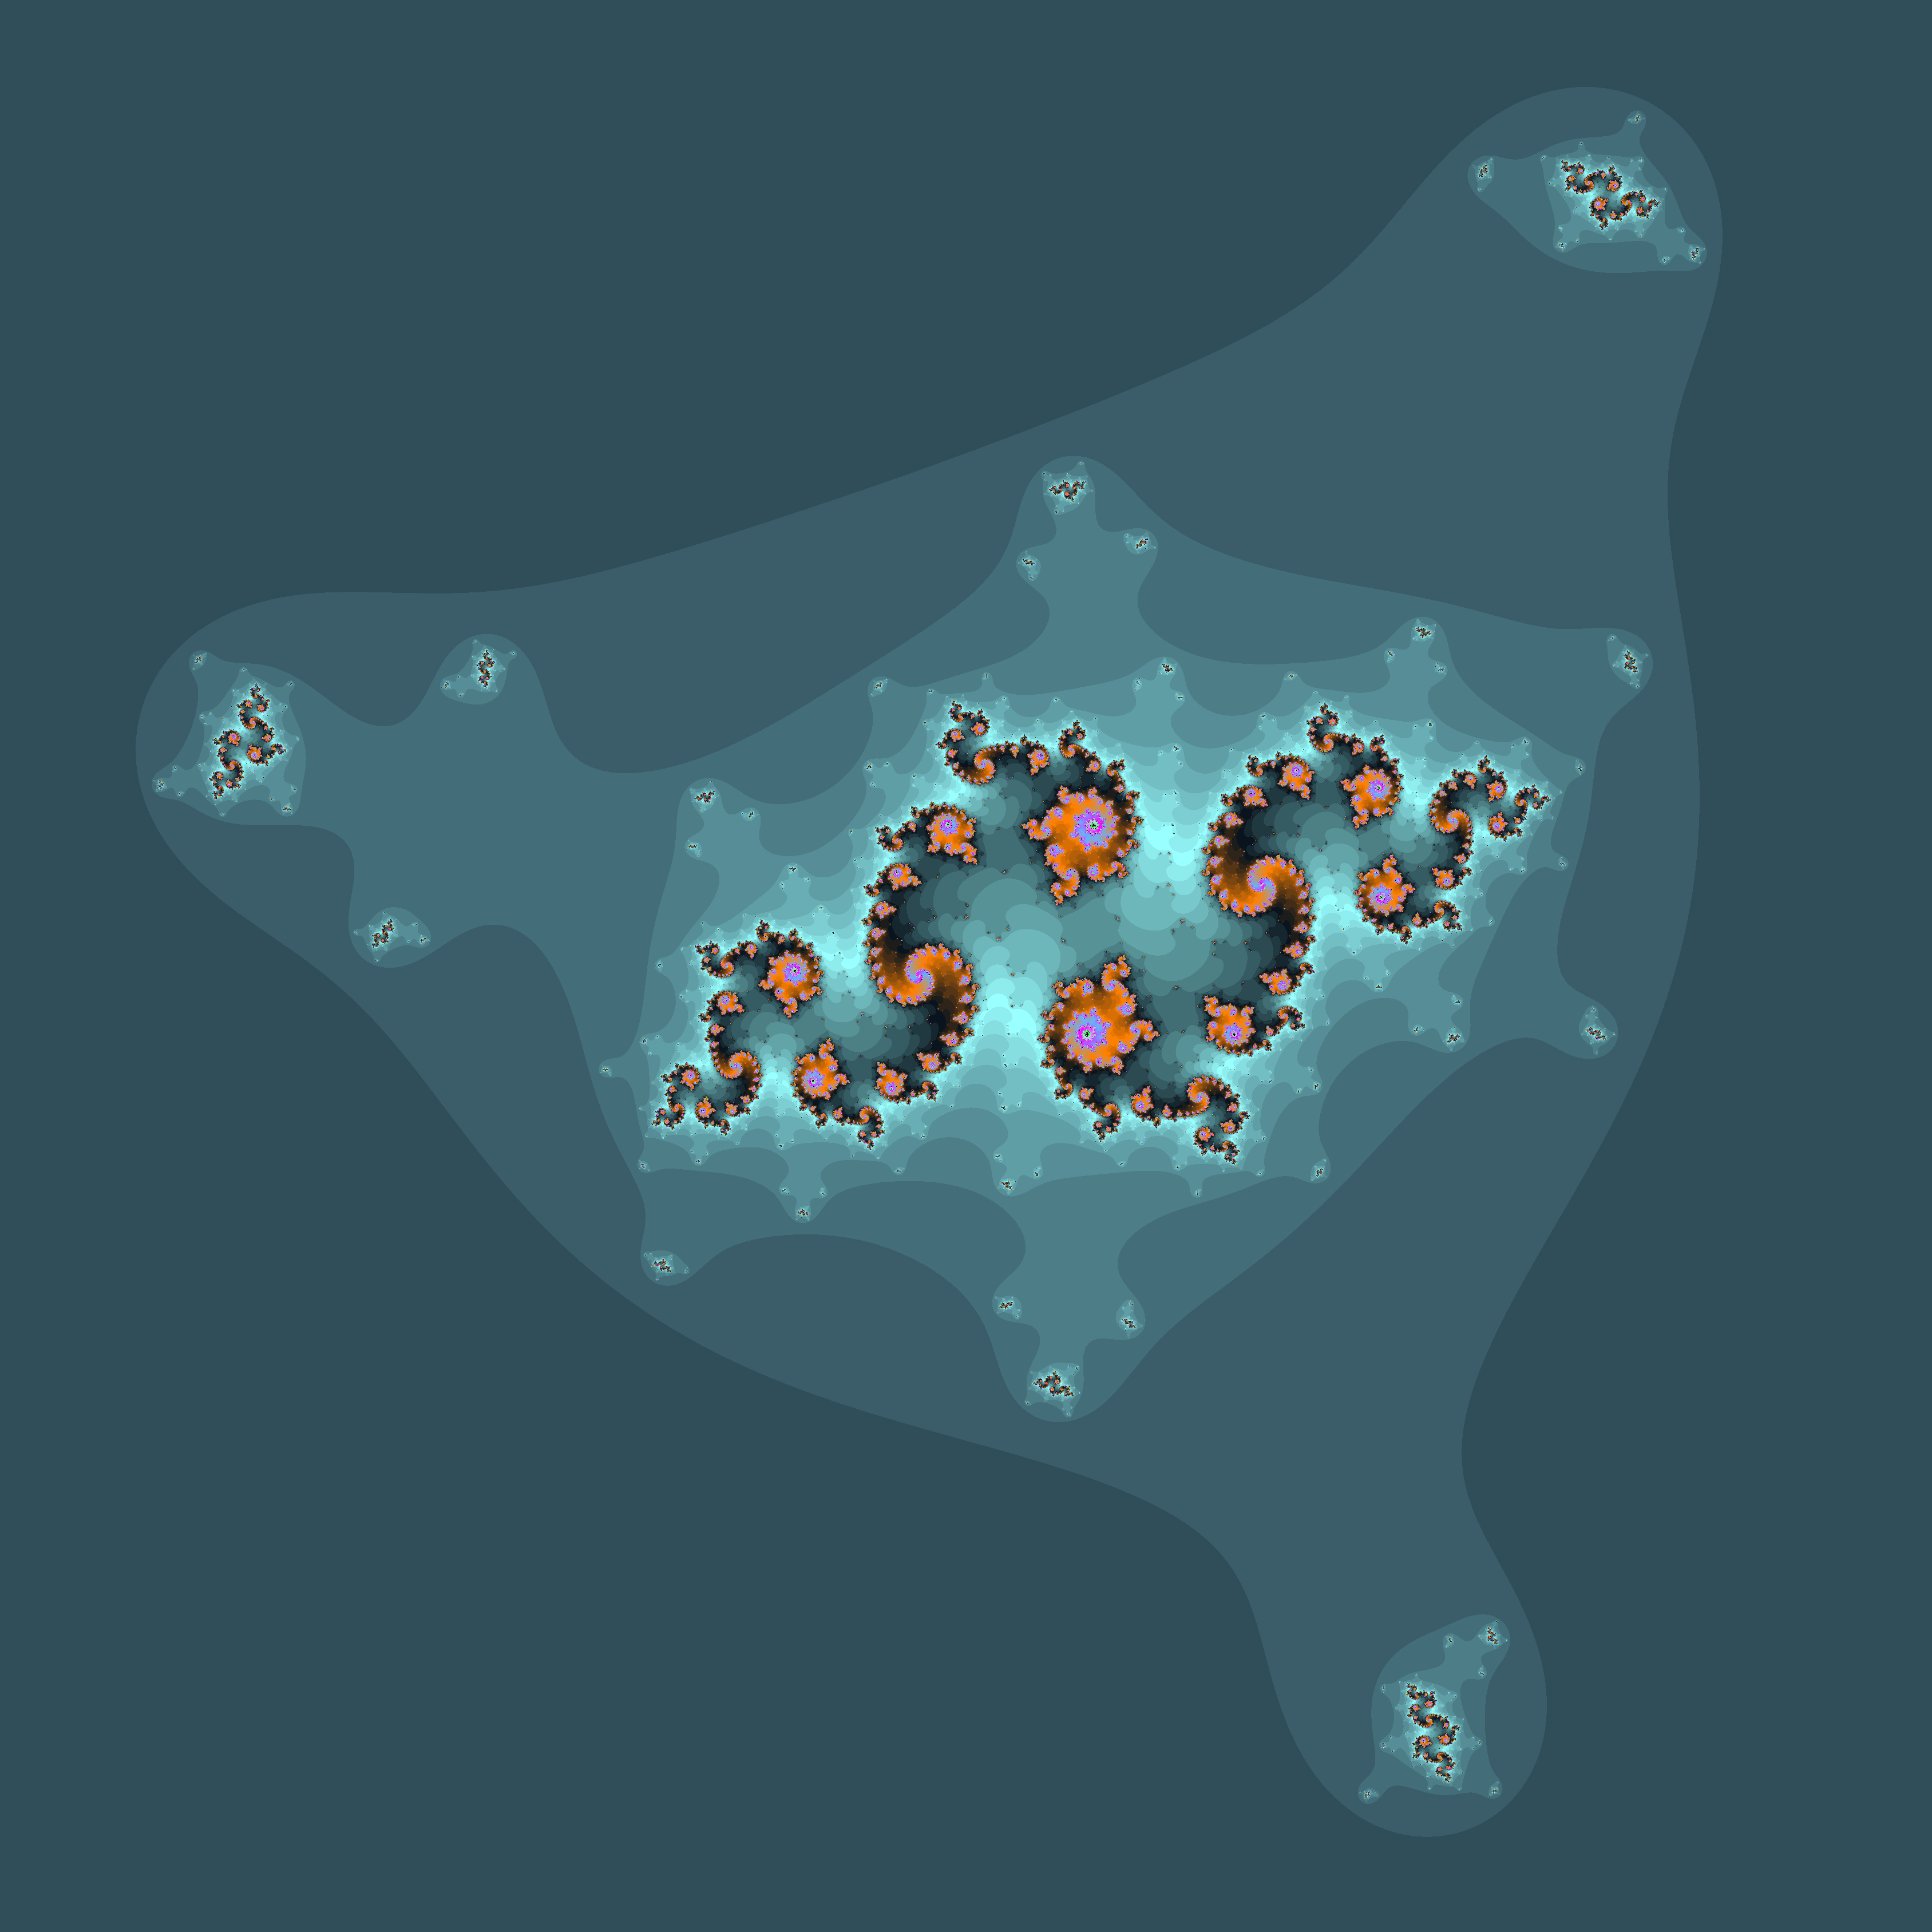
\includegraphics[width=6cm]{graphics/juliaEscapetime2.png}
\caption{
Mandelbrotova množica in napolnjena Juliajeva množica polinoma pete stopnje,
narisani z algoritmom Escapetime. 
Če levo sliko primerjamo s Sliko \ref{img:mandelbrotPlain}, opazimo izboljšavo v prikazani strukturi.
}
\label{img:Escapetime}
\end{figure}

Pomankljivost algoritma Escapetime je, da barve povežemo s skromnim naborom celih števil od $1$ do $K+1$,
zaradi česar se na zgornjih slikah vidi barvni prehod.
Očitna rešitev bi bila nastavitev višjega števila $K$, a je s tem povezan nepremostljiv problem,
da z višanjem $K$ dobivamo čedalje manj opazen rob.
\end{primer}
\vskip 2mm

V nadaljevanju nas bo zanimalo, kako bi lahko ta osnovni algoritem izboljšali. 
Konkretno, zanimalo nas bo, kako na učinkovit način podati oceno razdalje od neke točke $c \notin \M$ do $\M$.
Za izpeljavo te ocene bomo potrebovali naslednji klasični rezultat kompleksne analize. 
Njegov dokaz lahko bralec najde v \cite[Izrek~A.6.]{milnor}.

\begin{izrek}[Koebejev četrtinski izrek]\label{izr:Koebe}
Če je $f \colon \D \to \CC$ injektivna in holomorfna, potem 
$f(\D)$ vsebuje disk s središčem v $f(0)$ in radijem $|f'(0)| / 4$.
\end{izrek}

Spomnimo se Mandelbrot-B{\"o}ttcherjeve preslikave $\Phi$ iz Definicije \ref{def:MandelBottcher}.
Ta je po Izreku \ref{izr:DouadyHubbard} holomorfna bijekcija iz $\CC \smallsetminus \M$ v $\CC \smallsetminus \overline{\D}$.
Nadalje definirajmo preslikavo
\begin{equation*}
    G(c)= 
\begin{cases}
    \log(|\Phi(c)|), & \text{za } c \in \CC \smallsetminus \M, \\
    0,                   & \text{za } c \in \M,
\end{cases}
\end{equation*}
ki jo imenujemo {\em Douady-Hubbardov potencial}.
Dokaz leme \Ref{lem:expMandelBottcher} nam pove, da je $G$ zvezna z vrednostmi v $\R_0^+$.
Torej je potencial $G$ predpis, ki kompleksnemu številu priredi realno vrednost.
Za linearno aproksimacijo bo pomemben njen {\em Wirtingerjev odvod} po spremenljivki $c$, 
ki ga označimo kar z $G'(c)$ (glej Dodatek).

Izberimo $c \in \CC \smallsetminus \M$ in recimo, da je njej najbližja točka v $\M$ oblike $c + h$ za nek $h \in \CC$.
Potem je $G(c + h) = 0$,
po drugi strani pa je v Dodatku izpeljana tudi naslednja oblika linearne aproksimacije za našo funkcijo
$$G(c + h) \approx G(c) + 2\Real(G'(c)h).$$
Nadalje s trikotniško neenakostjo ocenimo
$$0 \approx |G(c) + G'(c)h| \geq |G(c)| - 2|G'(c)| \cdot |h| \implies |h| \gtrapprox \frac{G(c)}{2|G'(c)|},$$
kjer smo upoštevali, da je $G(c) > 0$.
Dobili smo aproksimacijo za spodnjo mejo oddaljenosti $c$ od $\M$,  ki pa je seveda dobra le takrat, ko je vrednost $|h|$ majhna.

Poiščimo še zgornjo mejo, ki pa bo tokrat neodvisna od $h$.
S predpisom 
$$g(w) := \log(\Phi(c + |h|w))$$
je na $\D$ podana holomorfna in injektivna preslikava.
To sledi iz tega, da je za $w \in \D$ vrednost $\Phi(c + |h|w)$ omejena stran od $\overline{\D}$, tam pa je $\Phi$ injektivna in holomorfna.
Zato lahko za $g$ uporabimo Izrek \ref{izr:Koebe} in dobimo, da $g(\D) \subset \CC\smallsetminus\{0\}$ vsebuje disk s središčem v $g(0)$ in radijem $|g'(0)| / 4$.
Če opazimo še, da je $\Real(\log(z)) = 0$ natanko tedaj, ko je $z \in \SSS$, dobimo neenakost v izrazu
$$G(c) = \Real(g(0)) > \frac{|g'(0)|}{4} = \frac{|h|}{4} \cdot \left|\frac{\Phi'(c)}{\Phi(c)}\right| 
= \frac{|h|}{2} \cdot |G'(c)| \implies |h| < \frac{2G(c)}{|G'(c)|},$$
kjer smo upoštevali, da je preslikava $\Phi$ holomorfna in zato
$$\overline{\Phi}'(c) = 0 \implies 2G'(c) = \frac{d}{dc} \; \log\left(\Phi(c)\overline{\Phi}(c)\right) 
= \frac{\Phi'(c)\overline{\Phi}(c) + \Phi(c) \overline{\Phi}'(c)}{\Phi(c)\overline{\Phi}(c)}
=\frac{\Phi'(c)}{\Phi(c)}.$$

Vidimo, da je smiselno definirati vrednost 
\begin{equation}\label{eq:defDc}
D_c := \frac{G(c)}{|G'(c)|} =  \frac{2 \cdot \log\left(|\Phi(c)|\right) \cdot |\Phi(c)|}{|\Phi'(c)|},
\end{equation}
saj zanjo velja, da se razdalja od $c \in \CC \smallsetminus \M$ do $\M$ giblje približno med $D_c/2$ in $2D_c$.
Naš naslednji cilj je podati enostaven postopek za izračun te vrednosti.
S tem v mislih definirajmo zaporedji $(\tilde{c_k})_k$ in $(d_k)_k$, s predpisi
$$\tilde{c}_k := q_c^k(c) \quad \text{in} \quad d_k := \frac{d\tilde{c}_k}{dc}.$$
Sedaj z upoštevanjem enakosti (\ref{eq:defDc}), limitne definicije za preslikavo $\Phi$ iz dokaza Leme \ref{lem:holMandelBottcher},
in elementarnih pravil odvajanja lahko izpeljemo enakost
$$
D_c = 2 \lim_{k\to\infty} \frac{\log(|\tilde{c}_k|) \cdot |\tilde{c}_k|}{|d_k|}.
$$
Torej potrebujemo le še vrednosti členov $d_k$.
Enostaven izračun le teh pa nam omogoča verižno pravilo, s pomočjo katerega dobimo rekurzivno zvezo
\begin{align*}
d_0 &= 1 \\
d_k &= 2\cdot \tilde{c}_{k-1} \cdot d_{k-1} + 1.
\end{align*}
Tako smo podali enostavne formule za izračun vseh vrednosti, ki jih potrebujemo za izračun števila $D_c$.
Kot smo že pripomnili, naša aproksimacija spodnje meje velja le za vrednosti $c$, ki so blizu $\M$.
Ker nas v glavnem zanima struktura blizu roba, to v našem primeru ne bo problematično.
Spodnji algoritem implementira naše ugotovitve.
\begin{small}
\begin{algorithmic}
\Function{DEM}{$c, K, M$}
	\State $k \gets 1$
	\State $\tilde{c}_k \gets c$
	\State $d_k \gets 1$
	\While{$k \leq K \algAnd \max\{|\tilde{c}_k|, |d_k|\} \leq M$}
		\State $d_k \gets 2 \cdot \tilde{c}_k \cdot d_k + 1$
		\State $\tilde{c}_k \gets \tilde{c}_k \cdot \tilde{c}_k + c$
		\State $k \gets k + 1$
	\EndWhile
	\If{$|\tilde{c}_k| \leq 2$} 
		\Return $0$
	\Else \
		\Return $2 \cdot \log(|\tilde{c}_k|) \cdot |\tilde{c}_k| \;/\; |d_k|$
	\EndIf
\EndFunction
\end{algorithmic}
\end{small}
Tu smo uvedli še pogoj, da morata biti člena $d_k$ in $\tilde{c}_k$ absolutno omejena z nekim velikim številom $M>0$.
To število predstavlja zgornjo mejo števil, s katerimi lahko operiramo, in tako preprečuje prekoračitev.

\begin{figure}[h]

\includegraphics[width=6cm]{graphics/mandelbrotDEM8.png}
\includegraphics[width=6cm]{graphics/mandelbrotDEM9.png}
\caption{
Celoten in približan del Mandelbrotove množice, narisana z algoritmom DEM.
Če primerjamo s Sliko \ref{img:Escapetime}, opazimo, da imamo sedaj izražen bistveno 
bolj gladek prehod barv, saj je zaloga vrednosti funkcije DEM teoretično zvezna množica.
}
\end{figure}

\noindent Omenimo še, da je bistvena izboljšava tega algoritma stabilnost,
saj višanje števila iteracij $K$ ne vpliva več tako zelo na izrazitost roba, 
temveč vrne le boljšo aproksimacijo razdalje.

Izkaže se, da lahko podoben premislek naredimo tudi za oceno oddaljenosti točk od povezanih napolnjenih Juliajevih množic.
Vzemimo polinom $p$ stopnje $d\geq2$, katerega Juliajeva množica je povezana.
Ker je njegova invertirana B{\"o}ttcherjeva preslikava $\phi_p \colon \CC \smallsetminus \J_p^\ast \to \CC \smallsetminus \overline{\D}$
po Izreku \ref{izr:FundamentalDichotomy} in Izreku \ref{izr:invBottcher} biholomorfna, lahko postopamo enako kot prej, 
le da zamenjamo Mandelbrot-B{\"o}ttcherjevo preslikavo $\Phi$ z invertirano B{\"o}ttcherjevo preslikavo $\phi_p$.
Tako definiramo
$$G_p(z) := \log(|\phi_p(z)|) = \lim_{k\to\infty} d^{-k}\log(|p^k(z)|).$$
Fiksirajmo $z \in \CC \smallsetminus \J_p^\ast$ in izračunajmo
$$
\frac{G_p(z)}{|G_p'(z)|} = 2 \lim_{k\to\infty}\frac{\log(|z_k|) \cdot |z_k|}{|d_k|},
$$
kjer označimo $z_k := p^k(z)$ in $d_k := dz_k / dz$. 
Spet za izračun $(d_k)_k$ upoštevamo verižno pravilo in tako dobimo rekurzivno zvezo
\begin{align*}
d_0 &= 1 \\
d_k &= p'(z_{k-1}) \cdot d_{k-1}.
\end{align*}
Algoritem je podoben prejšnjemu, le da zamenjamo izračun ustreznih zaporedij 
in za radij spet namesto $2$ vzamemo tega iz Trditve \ref{trd:escaperadius}.

\begin{figure}[h]

\includegraphics[height=4cm]{graphics/julia38.png}

\includegraphics[height=4cm]{graphics/julia64.png}

\includegraphics[height=4cm]{graphics/julia70.png}

\caption{
Povezane napolnjene Juliajeve množice, 
narisane z algoritmom DEM in uporabo različnih barvnih tabel.
}
\end{figure}

Po drugi strani za polinome z nepovezano Juliajevo množico sicer lahko uporabimo holomorfno razširitev B{\"o}ttcherjeve preslikave, 
a nimamo zagotovila, da je ta biholomorfna ali sploh injektivna.
Zato pri oceni ne moremo uporabiti Izreka \ref{izr:Koebe} in tako izpeljati zgornje meje razdalje.
Še vedno pa lahko izpeljemo spodnjo.

\begin{figure}[h]

\includegraphics[height=4cm]{graphics/julia30.png}
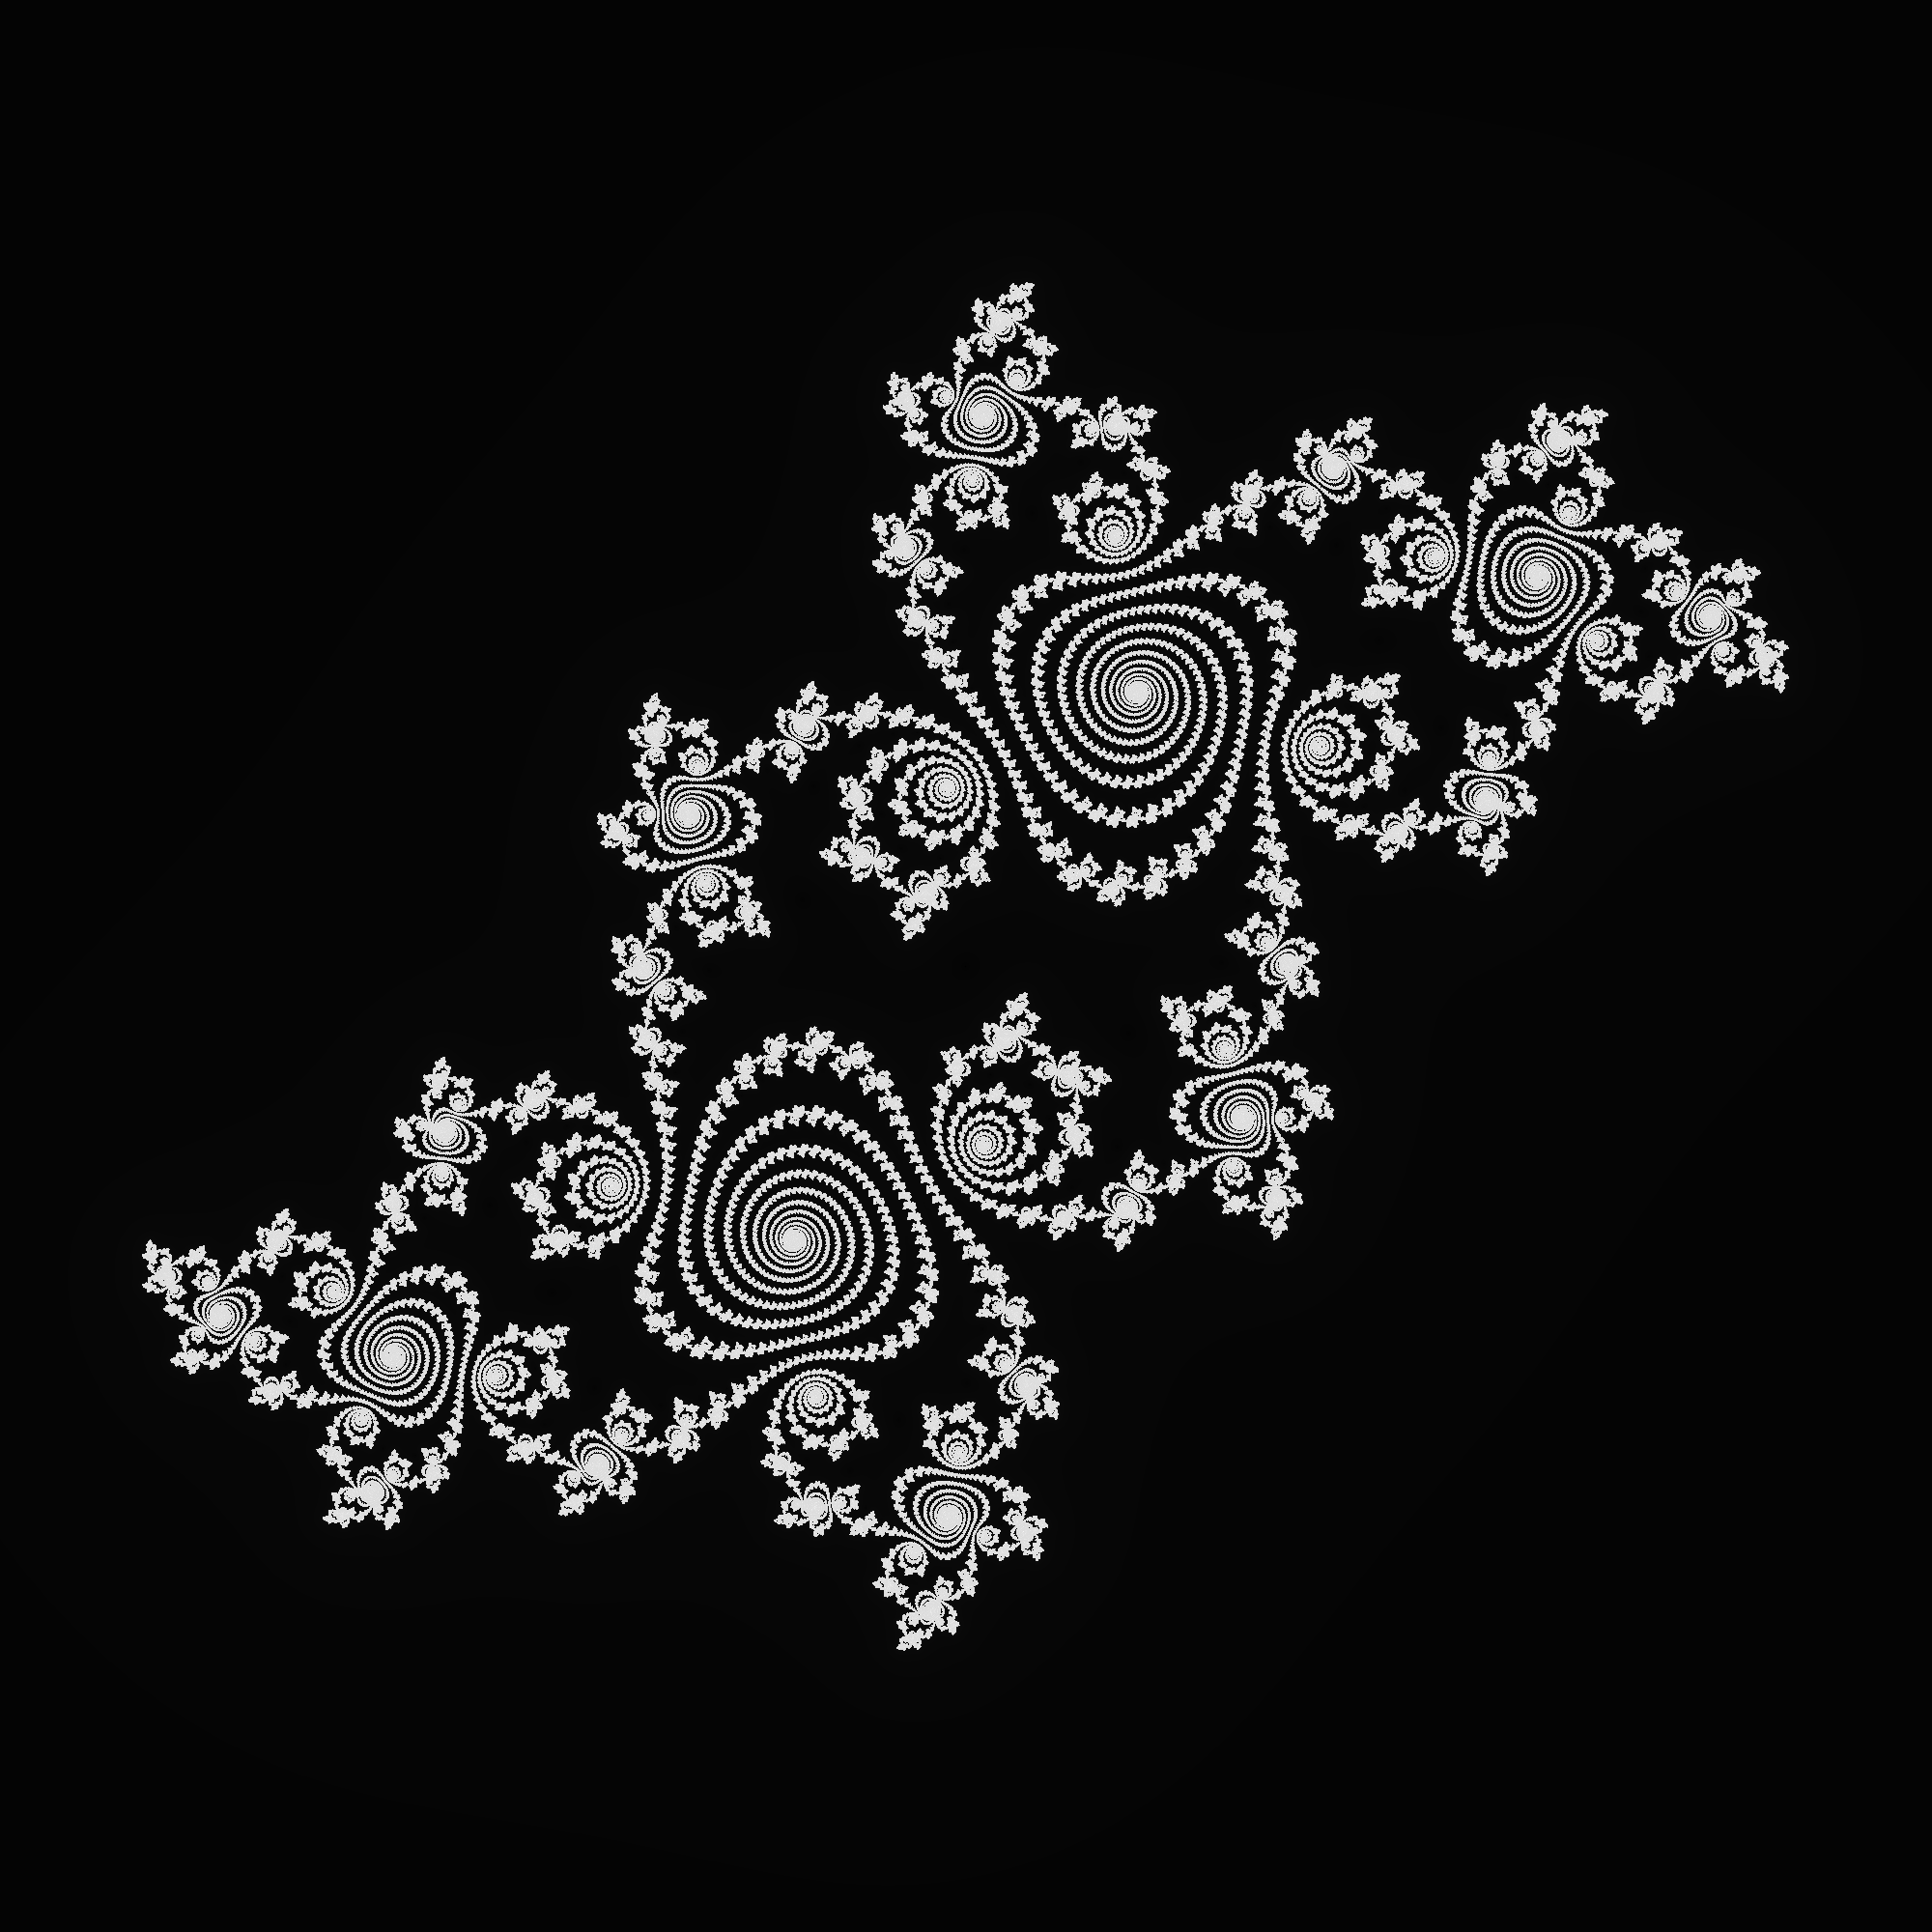
\includegraphics[height=4cm]{graphics/julia77.png}
\includegraphics[height=4cm]{graphics/julia58.png}

\caption{
Nepovezane napolnjene Juliajeve množice, 
narisane z algoritmom DEM in uporabo različnih barvnih tabel.
}
\end{figure}

Še enkrat opomnimo, da opisani algoritmi vrnejo le število, ki predstavlja nek podatek o relaciji med testno točko in množico.
Te podatke lahko še naprej transformiramo in na koncu prenesemo v sliko preko barvne tabele, definirane po želji.

\clearpage

\appendix
\section{Linearna aproksimacija kompleksnih funkcij}
Namen dodatka je pojasniti linearno aproksimacijo in odvod kompleksne preslikave,
katere realni in imaginarni del sta zvezno odvedljivi funkciji.
Vzemimo torej takšno kompleksno preslikavo  $G$, podano s predpisom
$$G(x + iy) = U(x, y) + iV(x, y).$$
Če enačimo bazo $(1, i)$ za $\CC$ s parom enotskih vektorjev $(e_1, e_2)$, ki tvori bazo $\R^2$, 
dobimo po standardni diferencialni teoriji z {\em Jacobijevo matriko} enakost
$$dG(x + iy) = G_x(x, y) dx+  G_y(x, y) dy.$$
Če uvedemo oznaki 
$$dz = dx + i dy \quad \text{in} \quad d\bar{z} = dx - i dy \quad \implies \quad
dx = \frac{dz + d\bar{z}}{2} \quad \text{in} \quad dy = \frac{dz - d\bar{z}}{2i},$$
lahko zapišemo 
\begin{align*}
dG(x + iy) &= (U_x(x, y) + iV_x(x, y))dx + (U_y(x, y) + iV_x(x, y))dy \\
&= \frac{1}{2}(U_x(x, y) + V_y(x, y) + i(V_y(x, y) - U_x(x, y)))dz \\
&+ \frac{1}{2} (U_x(x, y) - V_y(x, y) + i(U_y(x, y) + V_x(x, y))) d\bar{z}.
\end{align*}
Definirajmo sedaj tako imenovana {\em Wirtingerjeva odvoda}
\begin{align*}
\frac{dG}{dz}(z) &= \frac{1}{2}\left(U_x(x, y) + V_y(x, y) + i(V_y(x, y) - U_x(x, y))\right), \\
\frac{dG}{d\bar{z}}(z) &= \frac{1}{2} (U_x(x, y) - V_y(x, y) + i(U_y(x, y) + V_x(x, y))).
\end{align*}
Z njuno pomočjo lahko diferencial kompleksne funkcije zapišemo kot
$$dG=G_z dz + G_{\bar{z}}d\bar{z}.$$
Dejstvo, da je $G$ holomorfna, je ekvivalentno enakosti $G_{\bar{z}}(z)=0$. 
To pomeni, da je ničelnost druge enačbe ekvivalentna klasičnemu {\em Cauchy-Riemannovemu sistemu}. 
Podobno velja tudi za konjugacijo te enačbe. Torej, če je $G$ holomorfna, sledi $\overline{G}_z(z)=0$. 
Kakorkoli, pri izpeljavi algoritma imamo opravka z neholomorfno funkcijo, ki pa slika v množico realnih števil. 
To pomeni, da bosta oba njena odvoda neničelna, vendar pa bo obstajala tudi korelacija med njima. 
Posledično lahko prvi odvod po kompleksni spremenljivki označimo kar z $G'(z)$.
Z direktnim računom lahko preverimo, da za funkcijo z $G$ z realnimi vrednostmi velja
$$G_{\bar{z}}(z) = \overline{G'(z)}.$$
To pomeni, da za kompleksne funkcije z realnimi vrednostmi velja
$$dG(z) = G'(z)dz + \overline{G'(z)}d\bar{z} =2\Real(G'(z)dz).$$

\clearpage

\section*{Slovar strokovnih izrazov}

\geslo {Fixed point} {Fiksna točka -- točka definirana v Definiciji \ref{def:fixedPoint}}

\geslo {n-cycle} {$n$-cikel -- nabor točk, definiran v Definiciji \ref{def:nCycle}}

\geslo {Basin of attraction} {Baza privlačnosti -- odprta okolica, definirana v Opombi \ref{op:attBasinOpen}}

\geslo {Attracting fixed point} {Privlačna fiksna točka -- točka, definirana v Definiciji \ref{def:fixedPointTypes}}

\geslo {Repelling fixed point} {Odbojna fiksna točka -- točka, definirana v Definiciji \ref{def:fixedPointTypes}}

\geslo {Neutral fixed point} {Nevtralna fiksna točka -- točka, definirana v Definiciji \ref{def:fixedPointTypes}}

\geslo {Superattracting fixed point} {Superprivlačna fiksna točka -- točka, definirana v Definiciji \ref{def:superattractingFixedPoint}}

\geslo {B{\"o}ttcher coordinates} {B{\"o}ttcherjeve koordinate -- preslikava iz Izreka \ref{izr:Bottcher}}

\geslo {Inverted B{\"o}ttcher map} {Invertirana B{\"o}ttcherjeva preslikava -- preslikava, definirana v Definiciji \ref{def:invertedBottcherMap}}

\geslo {Filled Julia set} {Napolnjena Juliajeva množica -- množica, definirana v Definiciji \ref{def:Julia}}

\geslo {Julia set} {Juliajeva množica -- množica, definirana v Definiciji \ref{def:Julia}}

\geslo {Fatou set} {Fatoujeva množica -- množica, definirana v Definiciji \ref{def:Julia}}

\geslo {The fundemental dichotomy} {Osnovna dihotomija -- ime Izreka \ref{izr:FundamentalDichotomy}}

\geslo {The Douady rabbit} {Douadyjev zajec -- ime napolnjenih Juliajevih množic oblike kot ta na Sliki \ref{img:DouadyRabbit}}

\geslo {Mandelbrot set} {Mandelbrotova množica -- množica definirana v Definiciji \ref{def:Mandelbrot}}

\geslo{Escapetime} {Ubežni čas -- algoritem, opisan v Primeru \ref{pr:Escapetime}}

\geslo{DEM (Distance Estimation Method)} {DEM -- algoritem, opisan v zadnjem poglavju}

\clearpage

\begin{thebibliography}{0}

\bibitem{conway}
J.B.~Conway, \emph{Functions of one complex variable}, New York; Berlin, Springer-Verlag, druga izdaja, 1978.

\bibitem{kelley}
J.L~Kelley, \emph{General topology}, New York; Berlin; London; Paris; Tokyo, Springer-Verlag, 1975.

\bibitem{milnor}
J.~Milnor, \emph{Dynamics in One Complex Variable}, Annals of Mathematical Studies, Princeton University Press, Princeton, NJ, tretja izdaja, 2006.

\bibitem{beardon}
A.F.~Beardon, \emph{Iteration of rational functions}, New York; Berlin; London; Paris; Tokyo; Hong Kong; Barcelona; Budapest, Springer-Verlag, 1991.

\bibitem{stoll}
D. ~Stoll, \emph{A Brief Introduction to Complex Dynamics}, The University of Chicago Mathematics,
dostopno na \url{https://math.uchicago.edu/~may/REUDOCS/Stoll.pdf}.

\bibitem{shishikura}
M.~Shishikura, \emph{The Hausdorff Dimension of the Boundary of the Mandelbrot Set and Julia Sets}, Annals of Mathematics, Princeton University Press, 1998,
dostopno na \url{https://arxiv.org/pdf/math/9201282.pdf}.

\bibitem{wilson}
L.R~Wilson, \emph{Distance estimation method for drawing Mandelbrot and Julia sets}, [ogled 26.~8.~2020], dostopno na \url{http://www.imajeenyus.com/mathematics/20121112_distance_estimates/distance_estimation_method_for_fractals.pdf}.

\end{thebibliography}

\end{document}

